\documentclass[12pt]{article}

\usepackage[backend=bibtex]{biblatex}
\addbibresource{bibliography}

\usepackage{multicol}

\usepackage{amsfonts}
\usepackage{amsmath}

\usepackage{xcolor}
\usepackage{listings}

\usepackage{graphicx}
\graphicspath{ {./images/} }

\usepackage{nameref}

\usepackage{lscape}

\usepackage{subfig}

\usepackage[hidelinks]{hyperref}

\usepackage{datetime}


% ------------------------------------------------------------------------------
% tikz
% ------------------------------------------------------------------------------
\usepackage{tikz}
\usetikzlibrary{calc, arrows.meta, positioning, automata, shapes}

\definecolor{mGreen}{rgb}{0,0.6,0}
\definecolor{mGray}{rgb}{0.5,0.5,0.5}
\definecolor{mPurple}{rgb}{0.58,0,0.82}
\definecolor{backgroundColour}{rgb}{0.95,0.95,0.92}

\lstdefinestyle{CStyle}{
	backgroundcolor=\color{backgroundColour},   
	commentstyle=\color{mGreen},
	keywordstyle=\color{magenta},
	numberstyle=\tiny\color{mGray},
	stringstyle=\color{mPurple},
	basicstyle=\footnotesize,
	breakatwhitespace=false,         
	breaklines=true,                 
	captionpos=b,                    
	keepspaces=true,                 
	numbers=left,                    
	numbersep=5pt,                  
	showspaces=false,                
	showstringspaces=false,
	showtabs=false,                  
	tabsize=2,
	language=C
}

\title{Reachability analysis for continuous one-counter automata}
\author{Lars Van Roy\\
\textit{dept. of Mathematics and Computer Science} \\
\textit{University of Antwerp}\\
lars.vanroy@student.uantwerpen.be\\
\vspace*{10em}
Supervisor}

\newdateformat{monthyeardate}{\monthname[\THEMONTH], \THEYEAR}

\begin{document}
	
\begin{titlepage}
	\begin{center}
		\vspace*{1cm}
		
		{\Large\textbf{Reachability analysis for continuous one-counter automata}}
		
		\vspace{1.5cm}
		
		
\includegraphics[width=0.3\textwidth]{ua.jpg}
		
		\vspace{1.5cm}
		
		\textbf{Lars Van Roy}
		
		\vspace{0.5cm}
		
		\textit{dept. of Mathematics and Computer Science} \\
		\textit{University of Antwerp}
		
		\vspace{3cm}
		Supervised by \\
		Guillermo Alberto Perez \\
		Tim Leys
		
		\vspace{2cm}
		\monthyeardate\today
	\end{center}
\end{titlepage}

\begin{abstract}
\noindent
Reachability is an important metric and lack thereof is a known problem that can heavily affect the efficiency of code. It has been proven that reachability is decidable for continuous one counter automata which we will use in our approach. The proposed approach will provide a means to convert C code to continuous one counter automata followed by an algorithm which is capable of analysing the reachability of each of the nodes within the generated automata. This is an extension to existing research in which we already provided a means to perform the conversion from code to automata. 

The newly added approach to compute reachability will make use of reachability intervals, which will be used to represent the set of values which a conditional variable can be equal to at any point throughout the evaluation of the automaton. There will be two variations, one for parametric counter automata and for non-parametric counter automata.

Finally, we will apply the combination of approaches on an existing project called xrdp, as to determine the usefulness of the approach. This application resulted in a total of 33 functions being identified as analysable of which all were correctly identified as fully reachable. To ensure that non reachable cases can also be handled further manual evaluation was performed which resulted in correct identification for all considered cases.

\end{abstract}

\newpage
\tableofcontents

\newpage

\cleardoublepage
\phantomsection
\addcontentsline{toc}{section}{\listfigurename}
\listoffigures

\cleardoublepage <*-+/

\phantomsection
\addcontentsline{toc}{section}{\listtablename}
\listoftables

\cleardoublepage

\phantomsection
\addcontentsline{toc}{section}{\lstlistlistingname}
\lstlistoflistings

\newpage

\phantomsection
\addcontentsline{toc}{section}{Nederlandstalige samenvatting}
\section*{Nederlandstalige samenvatting}
Een gekend probleem bij het schrijven van code is het vinden van lijnen code die niet bereikbaar zijn \cite{713323, 10.1145/1292316.1292319}. Onbereikbare code kan veel oorzaken hebben maar één van de moeilijker te analyseren situaties zijn condities die nooit voldaan worden. In deze gevallen is de code omringd door de conditie niet bereikbaar en zou deze dus eigenlijk weg moeten. 

Niet bereikbare code is een probleem en kan zelfs kritiek worden in energie gelimiteerde omgevingen zoals ingebedde systemen \cite{embeddedefficiency}. In deze situaties is het vitaal dat onze code zo efficiënt mogelijk is en dus is er absolute nood aan een methode die niet bereikbare code kan detecteren.

Continue één counter automaten zijn hiervoor een zeer interesante oplossing, aangezien het bewezen is dat de bereikbaarheid aantoonbaar is voor deze automaton \cite{succintandparametriconecounter, danialandjoel, blondin2021continuous}. In dit onderzoek zullen we een praktische implementatie geven voor de theoretische werkwijze gegeven door Michael Blondin et al. \cite{blondin2021continuous}. Deze theoretische implementatie was specifiek opgezet om gebrek aan bereikbaarheid te kunnen aantonen.

De beperking om maar één parametrische klok (of counter) toe te staan heeft een groot effect op het bereik aan code dat we kunnen analyseren. Dit is echter onvermijdelijk aangezien er geen bewijs is voor de bereikbaarheid van continue automaten met twee counters. Voor drie counters en meer is er bewezen dat dit niet beslisbaar is \cite{FEARNLEY201526}.

In dit onderzoek zulen we een werkwijze geven om C code om te zetten naar continue één counter automaten. Gebruik makend van deze gegenereerde automaten zullen we analyseren of er in deze code lijnen zijn die niet kunnen bereikt worden. Dit zal gebeuren aan de hand van de volgende stappen:

\begin{enumerate}
	\item Voer pre analyse uit en analyseer alle compiler specifieke code
	\item Converteer de C code naar een parse tree met behulp van ANTLR
	\item Voer context vrije reducties uit op de parse tree
	\item Voer context sensitieve reducties uit op de parse tree
	\item Verifieer of de parse tree converteerbaar is naar een automaat
	\item Genereer de automaat
	\item Analyseer de bereikbaarheid
	\item Raporteer onbereikbare code indien deze gevonden is
\end{enumerate}

De code zal, buiten het feit dat deze maar één conditionele variabel kan hebben, ook beperkt worden in de operaties die hierop kunnen uitgevoerd worden. Aan een conditionele variabel kunnen enkel constante of parametrische waarden toegewezen worden of combinaties van sommen en aftrekkingen met constante of parametrische waarden. De conditionele waarde mag verder enkel met parameters of constante waarden vergeleken worden met de condities is gelijk aan, is niet gelijk aan, is strikt kleiner dan, is kleiner dan, is groter dan en is strikt groter dan. Ten slotte mogen de parameters zelf nooit aangepast worden tijdens de evaluatie van de functie.

Niet alleen de functie inhoud maar ook de definitie zal een beperking krijgen, zo accepteren we enkel parameters van het type integer.
\newpage
\section{Introduction}
A well known problem in writing code is determining whether or not every line of code is reachable. It is often impossible to properly determine whether or not a line of code guarded by a conditional statement is going to be reachable in any possible execution of the code \cite{713323, 10.1145/1292316.1292319}. Unreachable code is never desired and is an ever more pressing issue for energy restrained environments such as embedded computer systems \cite{embeddedefficiency}. In these systems, we want our execution to be as efficient as possible, and therefore avoid conditions that can never be satisfied or lines that can never be reached. To remedy this, a proper unreachable code detection approach is needed.

In order to analyse the reachability, we will make use of the fact that code is easily convertible to automata. All statements within the code that are related to counter updates can directly be converted to operations within an automaton. Each line of code can be represented by one or more nodes and a traversal of an automaton can be directly linked to the traversal of the code itself.

Continuous one counter automata are especially interesting as it has been proven that reachability is decidable for this type of automata \cite{succintandparametriconecounter, danialandjoel, blondin2021continuous}. In this paper we will provide a practical implementation for the theoretical approach that was provided by Michael Blondin et al.\cite{blondin2021continuous} which can be used to prove reachability of nodes. 

Adding the restriction of only allowing a single parametric clock has a big effect on the types of code we can analyse. However, this is unavoidable, since there is no proof for continuous two counter machines. Three counter machines and up have been proven to be undecidable \cite{FEARNLEY201526}.

In this paper we will provide the overview of an approach which will convert C code to a continuous one counter automaton. Using the result of this first step, we will then provide a means to analyse the reachability of any of the nodes of said automaton. The following steps are taken without our approach to prove the existence of dead code.

\begin{enumerate}
	\item Perform pre analysis to resolve all C macro's
	\item Convert C code into a parse tree, using ANTLR
	\item Perform context free reductions on this parse tree
	\item Perform context sensitive reductions on this parse tree
	\item Validate the resulting parse tree, to be conforming to the code constraints
	\item Generate the counter automaton
	\item Analyse which nodes are reachable
	\item Link potential unreachable statements back to the lines within the original code base
\end{enumerate}

The code can at most contain one counter and for the continuation of this paper we will only consider examples where this holds. Cases with no counter will not be considered as these are assumed to be trivial. Furthermore, the operations on the counter will be restricted, the counter can only be updated via assignments with parameters or constants, and the counter can only be compared using equality, inequality, strict less than, strict greater than, less than or equal, greater than or equal, and only to parameters or constants. As a final code constraint, the function parameters are not allowed to be altered throughout the duration of the code.

Other than the described code constraints, functions must have integer parameter types (if any) to be converted into a counter automaton.

\subsection{Research questions}
The objective of this research can be summarised in two core research questions:

\begin{description}
	\item[Question 1: ] \hfill \\ Can we practically determine the reachability of continuous one counter automata?
	\item[Question 2: ] \hfill \\ Can we identify dead code in software written in the C language by analysing the reachability of the corresponding counter automata?
\end{description}

To solve these questions we will give two different approaches that are capable of determining reachability of nodes in both parametric and non-parametric one counter automata. Both approaches will additionally be applied to xrdp, a project used to login to remote machines that is entirely written in C. 

The solution to the questions above can be divided into three different steps, where the final step will be further divided in two different solutions.\\
\\
\noindent
\textbf{Convert the C code to a one counter automaton} \\
This approach was previously done in a separate research but the general approach will be repeated here. It will furthermore be modified and perfected as an improvement of the existing work. This approach will be discussed in Section \textit{\ref{sec:generation} \nameref{sec:generation}} in which we will discuss the different steps part of converting C code.\\
\\
\noindent
\textbf{Specify a textual format for automata to allow reading and writing of automata}\\
The result of the previous step will be stored using the dot format which is part of Graphviz \cite{10.1007/3-540-45848-4_57}. This input should be readable to perform the reachability on it. We furthermore want to be able to provide this approach as a stand-alone concept, thus allowing the reachability analysis to be performed on arbitrary automata without the coupling with the compiler. In the Section \textit{\ref{sec:automaton input} \nameref{sec:automaton input}} we will discuss the steps needed to read an automaton from a dot file.\\
\\
\noindent
\textbf{Perform reachability analysis on non-parametric continuous one counter automata} \\
The first reachability analysis approach will be used to analyse the reachability of non-parametric continuous one counter automata. This implies that there can never be any operation applied to a counter with parameters involved. This approach will iteratively go through the automaton by making use of reachability intervals. The different steps and operations will all be discussed in detail in Section \textit{\ref{sec:reachability non parametric} \nameref{sec:reachability non parametric}}.\\
\\
\noindent
\textbf{Perform reachability analysis on parametric continuous one counter automata} \\
A secondary approach for reachability analysis will be given in Section \textit{\ref{sec:reachability parametric} \nameref{sec:reachability parametric}}. This approach will estimate the reachability intervals which were also used for the non-parametric variant. We will define conditions on the intervals and employ a SAT solver to guess a valid reachability interval configuration. The SAT solver will also support parametric automata and this approach will therefore be used as an alternative to the first approach in case the function uses parameters.

\section{Motivation}
Code efficiency is one of the core aspects on which the quality of code is measured. Inefficient code can incrementally lead to a slower product, even though it only represents a small part of a much larger whole. This is because code reuse is a critical aspect in Object Oriented Programming (OOP) \cite{10.1145/71605.71612}. In OOP we tend to write code by encapsulating it within classes (objects) based on the functionality they provide. This allows us to simply reuse that object whenever we need that specific functionality. As a direct result of this, every time we introduce code inefficiency, this will get replicated whenever we need use of the specific functionality in which the inefficiency was introduced.

Code inefficiency can also indirectly affect other projects. Many languages such as C, C++, Java and Python support the option to introduce libraries. These libraries are other projects which will entirely be introduced within the current project as to prevent the need to add a new implementation for a functionality which has already been implemented elsewhere. The same effect can occur here where an inefficiency within the library will get propagated to the other projects which make use of said library. As a means to speed up development there are even tools such as Hunter \cite{10.1145/2950290.2983934} which are intended to query large code bases to find code which already implements the feature that is needed, thus increasing the likelihood of using existing code.

One of the contributors to the efficiency of code is the reachability of code. Dead code implies that there is a piece of code that can never be reached and is thus useless. This might be due to a certain function simply never being invoked and in most cases this will not affect the actual efficiency of the code as this is trivially filtered out by compilers. However, guarded (conditional) pieces of code can be an issue in case they are not satisfiable. This can not simply be resolved by a compiler nor will it always get caught by all IDE's (Integrated Development Environment). A dead conditional statement will get evaluated every time said piece of code is used and can therefore contribute to a major efficiency reduction considering the code reuse that was mentioned above.

Popular IDE's do already implement reachability analysis up to a certain degree. However, the dead code elimination they perform is shallow and limited. The code example given below was executed using Clion and Eclipse, two of the more commonly used C IDE's. While it is known that both can find some dead code, it was not able to resolve this case, where the condition on line 4 can never evaluate to true. This is because the for statement on line 3 will always prevent line 4 from evaluating to true and yet they did not detect this.

\begin{lstlisting}[style=CStyle, caption={Example C code where Eclipse and Clion would not identify dead code.}]
bool is_mul(int a, int b) {
  int temp = b;
  for(; temp > 0;){
    if(temp == 0){
      break;
    }
    temp -= a;
  }
  return temp == 0;
}

int main() {
  printf("5 is a multiple of 2: %d\n", is_mul(2, 5));
  printf("6 is a multiple of 2: %d\n", is_mul(2, 6));
}
\end{lstlisting}

The approach provided within this paper will be able to detect this, as it can simply evaluate the possible values with which line 5 can be reached, it will result that there is no sequence in which line 5 can be reached and we can therefore conclude that the condition surrounding this statement can never be satisfied.

In the past research has been done regarding dead code analysis. In 1994 there was a research done by Jens Knoop et al. \cite{10.1145/773473.178256} where they attempted to analyse partial dead code. Partial dead code is code that is only dead in some of its execution paths. It will aim to resolve this by changing the branching structure or the semantics of the program which will result in the bit of code no longer being dead in any program path. This resolves one of the cases that is not touched by the approach prescribed within this paper and they can therefore both provide benefits to projects without any redundancy in evaluation.

A different research has been done on the analysis of the data model behind software in an attempt to identify dead code at the declaration level. This was done in 1997 by Yih-Farn R. Chen et al. \cite{10.1145/267896.267924} and was applied on C++ projects. It concluded by showing that it was in fact capable of identifying a significant amount of dead functions and variables. This is however on a different level than the current research will work on. The research in question did analysis on the data model and might have therefore missed a significant amount of dead code that was introduced within the code itself.

As can be concluded from the examples given above, there has been research on dead code analysis. This research is however dated and it did not specifically cover the environment which we will cover within this research. It is furthermore shown that within the majorly used IDE's such as Eclipse and Clion the cases which we will attempt to detect with this new approach are not yet covered. We can conclude that this research brings additional value to what is known about dead code analysis and can further enhance the optimization of software.
\section{Preliminaries}
This paper will make use of counter automata and more specifically continuous one counter automata. These automata are derived from the general definition of automata and signify an extension by adding the notion of counters.

\subsection{General automata}
The automata used in this research are a specific subset of the generally defined automata. The general definition for an automaton A is given by the tuple (Q, $\Sigma$, $\delta$, $q_0$, F) where
\begin{itemize}
	\item Q is the set of states
	\item $\Sigma$ is a finite set of symbols, called the alphabet of the automaton
	\item $\delta: Q \times \Sigma \rightarrow Q$ is the transition function
	\item $q_0 \in Q$ is the initial state
	\item $F \subseteq Q$ is a set of states of Q defining the final states, 
\end{itemize}

\subsection{Continuous one-counter automata}
A continuous one-counter automaton (COCA) is defined as a tuple $\mathcal{A}$ = $(Q, q_0, T, \tau)$ where
\begin{itemize}
	\item $Q$ is a finite set of states
	\item $q_0 \in Q$ is the initial state
	\item $T \subseteq Q \times op \times Q$ is the transition relation with $op$ the set of operations
	\item $I$ is a representation of all intervals over $\mathbb{Q}$
	\item $\tau: Q \rightarrow I$ is the mapping of the reachability intervals
\end{itemize}

At all times the automaton will be in a configuration $(q, c)$ where $q \in Q$ and $c$ the counter valuation where $(q_0, 0)$ is the initial configuration. The counter valuation $c \in \mathbb{N}$ represent one single value for which the counter is evaluated. We are interested in the reachability sets for each state q where the reachability set for q is $\{v | (q, v) \text{ is a reachable configuration}\}$.

The $\tau$ parameter represents a function that maps all nodes to their corresponding bounds. For a counter value to be part of the reachability interval of a node, it must respect the bounds implied by the $\tau$ function. The $\tau$ entry for a node q is represented by the an interval $[\underline{\tau(q)}, \overline{\tau(q)}]$ where $\underline{\tau(q)}$ and $\overline{\tau(q)}$ represent the lower and upper bounds of a node respectively.

The set of supported constraints within our evaluation are visualised by the $cond$ set below with $\epsilon$ representing the empty condition. Note that this is not binding for the code that we can analyse, several conditions might be convertible to constructs using only supported statements.
\[
cond = \{\leq c, =c, \geq c, \leq p, =p, \leq p: c \in \mathbb{N}, p \in P\} \cup \{\epsilon\}
\]

Parametric counter automata, as compared to regular counter automata, allow counters to be modified by parameters as well as constants. As the counters are assumed to be integers, we will only allow integer type parameters. We will consider the following set of allowed operations where $P$ is the set of parameters, the $\epsilon$ symbol will be used to represent an empty label.
\[
op = \{+c, -c, +p, -p: c \in \mathbb{N}, p \in P\} \cup \{\epsilon\}
\]

The final state is omitted from this definition as we are not interested in this. In general the reachability of every line of code will be under scope and not just a single one. Furthermore, making the assumption that the final state is the only state of which we want to analyse reachability creates a significant reduction in the use cases of this approach, and was therefore discarded.

\subsection{COCA reachability}
In this section we give an overview of how we approach the concept of reachability. The provided concept was proven by Michael Blondin et al. \cite{blondin2021continuous} and will be the basis for the remainder of the approach.

Throughout the evaluation we will be tracking the reachability interval(s) of all nodes denoted by $reach(q)$. $Reach(q)$ will represent the set of possible counter values c that can exist in a configuration $(q, c)$.

A $run\;\rho$ is a sequence of configurations $(q_0, v_0)(q_1, v_1)...(q_n, v_n)$ such that the following holds with $T$ the set of all transitions:

\begin{itemize}
	\item $\forall i \in [0, n)\;\exists \alpha \in (0, 1]\;\exists t \in T: (q_i, v_i) \xrightarrow{\alpha\;t}(q_{i+1}, v_{i+1})$
	\item $\forall i \in [0, n]: v_i \in reach(q_i)$
\end{itemize}

A state $q_i$, and thereby represented line $l$, will be considered reachable if there exists a $run\;\rho$ with the sequence $(q_0, v_0)(q_1, v_1)...(q_i, v_i)$. We can therefore convert the reachability of lines of code to the the following problem. \\
\\
\noindent
\textbf{COCA reachability:} \\
Given a COCA $\mathcal{A}$, an initial configuration $(q_0, v_0)$ and a target configuration $(q_n, v_n)$ does there exist a run $\rho = (q_0, v_0) ... (q_n, v_n)$?\\
\\
In this paper we will give two different approaches that will approximate the $reach(q_i)$ intervals for each node $q_i \in Q$, thus attempting to prove whether or not such a run exists. This is equivalent as the following results from the definition given above:

\begin{itemize}
	\item $reach(q_i) \neq \emptyset \rightarrow \exists \rho = (q_0, v_0) ... (q_i, v_i)$
\end{itemize}

\section{Analysis of dead code in C}
The approach given within this paper consists out of two major phases. The first phase will consist of the conversion from C code to one counter automata. The second phase will use the result from the first phase, and perform a reachability analysis on these generated automata. The first phase was already covered in preceding research and the majority of the notes on the approach in the first phase were taken from that research. They were copied here as this research will conclude the unfinished work that was done there, as well as make continuous references to the flaws which arose from it.

\begin{figure}[b]
	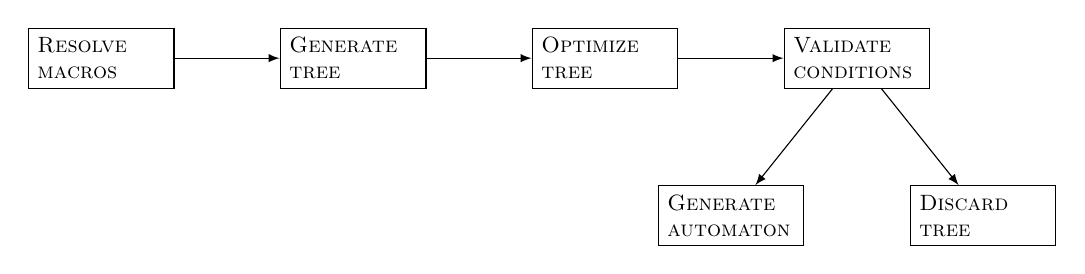
\begin{tikzpicture}[auto, >=latex, font=\footnotesize\scshape]
	\tikzstyle{center} = [draw=black, rectangle, text width=4.6em]
	
	\node[center]	at (0, 0) 		(q0) 	{Resolve macros};
	\node[center]	at (3.2, 0)		(q1)	{Generate tree};
	\node[center]	at (6.4, 0)		(q2)	{Optimize tree};
	\node[center]	at (9.6, 0)	(q3)	{Validate conditions};
	\node[center]	at (8, -2)		(q4)	{Generate \\automaton};
	\node[center]	at (11.2, -2)		(q5)	{Discard \\tree};
	
	\path[draw][->] 
	(q0) edge (q1)
	(q1) edge (q2)
	(q2) edge (q3)
	(q3) edge (q4)
	(q3) edge (q5);
	
	\end{tikzpicture}
	\caption{Overview of the automaton conversion process}
\end{figure}

The first step of the conversion will be the preprocessing step in which all c compiler macro's will get resolved.

Next, the second step starts with an initialization, which consists of the generation of a parse tree. This will be done using the default C grammar, with the extension of the boolean type as this is not within the C language by default.

Using the resulting parse tree we will perform a simple context-free optimization where we will remove all needless nodes. This is done as an intermediate step as it will allow us to make assumptions in the second part of the optimization, where we will do a more in depth optimization cycle. This second part will perform optimizations based upon the context in which the nodes appear, and will try to simplify the syntax tree as much as possible. The resulting tree will contain no more potentially ambiguous nodes and all remaining nodes will be those relevant in the remainder of the evaluation.

The fourth step will be an analysis on whether or not the resulting abstract syntax tree conforms to all earlier specified requirements and, if this is the case, we will continue with the fifth step, which will be the generation of the counter automaton. 

For a function to conform the arguments (if any) must be of type integer and must never be mutated within the function body, there can only be one counter and the counter can only be mutated using the operations part of the $op$ set displayed below.
\[
op = \{+c, -c, +p, -p, \leq c, =c, \geq c, \leq p, =p, \geq p: c \in \mathbb{N}, p \in P\} \cup \{\epsilon\}
\]

The generation of the automaton within the fifth step is done by traversing the tree and converting every statement that is directly relevant to the counter modifications to their corresponding automaton labels.

\subsection{Preprocessing}
\label{sec:conversion}
The program will start by resolving all the compiler macros that are part of C. These are intended to be resolved by the compiler at compile time, and are often dependent on which compiler was chosen/the environment on which the code is executed. For our use case I decided to select the global variables in such a way that these represent a windows machine that is using 64 bits. This is however not at all restricted to that and could further be expanded to support any environment and any combination of global variables possible. This selection is in essence not relevant as it should not affect the presence of dead code.

Something else that is part of these macros are the include statements. These statements were partially resolved in the sense that only the imports from the current project were handled. Includes from global C libraries are not relevant for the type of dead code elimination we attempt to do within this project and we therefore decided that the addition of said libraries would only result in a much larger code base to be analysed without any additional benefits for the dead code analysis of the actual project.

The if/elif/else macros were simply resolved by converting them to boolean expressions which can then be resolved by any boolean solver. These macro's are intended to identify whether or not global variables are defined and/or are of a current value and are thus relatively simple to resolve.

Finally, the define and undefine macros were resolved by simply tracking the values they defined and/or undefined throughout the evaluation of the code. 

\subsection{Initialization}
Using the flattened result of the preprocessor, the next step will start by running the generator ANTLR compilation unit on the given C code. In case there are any issues regarding simple compilation rules, the program will exit with an error, indicating the issues in the code. For the remainder of the execution, the code is assumed to be correct, and there will be no regard for potential issues within the code itself.

\subsection{Context-free abstract syntax tree generation}
Using the parse tree resulting from the ANTLR compilation, we will try to generate an abstract syntax tree that is as simple as possible without regarding any context. 

First of all, the code uses the notion of a node stack. This node stack will be used to store the nodes that are currently being evaluated.

The first loop will operate as a visitor, which will traverse the parse tree in a depth first manner. The first discovery of a node is done by calling the enter function corresponding to the type of node. As soon as all children of said node have been evaluated, the corresponding exit function will be called. 

However, the creation of nodes is not the same in all situations, in some cases, a specific kind of node will be created and in other cases it will not, depending on the rule used for the current node (which we can determine from the context of the current node). In order to know whether or not we need to pop a node from the node stack, we will allow the code to look at the top node in the stack, and evaluate the type of set node. No other context related evaluations will be allowed.\\
\\
\noindent
\textbf{Context-free analysis assignmentExpression example}\\
To look at a concrete example, consider the following rule in the grammar:
\begin{align*}
	&assignmentExpression\\
	&\text{:}\indent \text{conditionalExpression}\\
	&|\indent \text{unaryExpression assignmentOperator assignmentExpression}\\
	&|\indent \text{Digitsequence}; \\
\end{align*}
The rule for conditionalExpression needs to be there, as there is a chain of expressions, and some expressions need to be higher in the order than others, therefore all expressions with a higher priority need to be evaluated before the lower priority expressions. This is done by adding a rule to a lower priority expression in each expression class. It is however undesirable for these nodes to be added. Without regard for context in other nodes, we can simply look at the current node to see whether or not the conditionalExpression line is used (which ANTLR generated context allows us to do).

Since there is a chance no new node was added within the enter function, we will also be required to evaluate the top of the stack, to see whether or not the top of the stack is a node we need to pop, the code will do the same check that was done in the enter function of the traversal.

\subsection{Context-sensitive abstract syntax tree reduction}
There is still the need for reductions. We will attempt to implement constant propagation and substitution, in which we compute constant expressions, and replace variables with known value, by their actual value. Furthermore we will try to rephrase expressions by expressions with the same meaning, so that all expressions, if possible, are in an acceptable format for the counter automaton.

The context-sensitive reduction will also keep track of a lot of data about the variables in a symbol table. It will track whether or not variables are current initialized with a known value, values at certain points within the execution, it will track struct, union and enum definitions used for folding and so on. It will keep track of the kind of variables we have (eg. counters and parameters). All of this info will be used to enable the operations this cycle will perform, but will also be used in the validation loop.

The program will do this by traversing the abstract syntax tree resulting from the previous step, but will now specifically go through the children of relevant expressions (eg. assignment expressions, additive expressions, ...).

Important to note is that no folding/substitution will occur within loops, as these operations occur a variable number of times, and since there is no way of determining the exact number of times without evaluating the expression, this is considered too complex and often impossible, as counters may depend on parameters, which need to be chosen at evaluation time.\\
\\
\noindent
\textbf{Context-sensitive reduction example: constant propagation}\\
Another example of a needed reduction, is constant \textit{propagation} and \textit{folding}. It is possible that a code segment would initially be rejected, due to use of unwanted variables, while in essence, these variables are nothing but variable representations of results of constant expressions. By \textit{folding} we will attempt to simplify constant expressions by replacing them with their results. Once simplified to a constant value we will then attempt to \textit{substitute} the variables by replacing further uses with said value.

Consider the code in Listing \ref{lst:divide} below. It would initially be rejected, because the \textit{counter} variable is initialized with a value that is neither a constant nor a parameter.

\begin{lstlisting}[style=CStyle, caption={Example of a function in need of constant propagation}, label={lst:divide}]
bool divide(int p, int n){
	int variable = 5;
	variable += 20;
	int counter = variable;
	while(counter > 0){
		counter -= n;
	}
	counter += 1;
	counter -= 1;
	if(counter == 0){
		return true;
	}
	return false;
}
\end{lstlisting}

However, due to constant propagation and folding, we can simplify the two statements on line 2 and line 3, so that they become one simplified operation. This can be seen in Listing \ref{lst:dif variable}.

\begin{lstlisting}[style=CStyle, caption={Result of simplifying operations on \textit{variable}}, label={lst:dif variable}]
int variable = 25;
\end{lstlisting}

Now that \textit{variable} is just a constant, we can substitute its value which leads us to the situation given in Listing \ref{lst:sub variable}.
\begin{lstlisting}[style=CStyle, caption={Result of substituting \textit{variable}}, label={lst:sub variable}]
int variable = 25;
int counter = 25;
\end{lstlisting}

Now \textit{variable} has no further benefit for the execution and will be dropped. 

\begin{lstlisting}[style=CStyle, caption={Final version of the simplified function}, label={lst:divide final}]
bool divide(int p, int n){
	int counter = 25;
	while(counter > 0){
		counter -= n;
	}
	counter += 1;
	counter -= 1;
	if(counter == 0){
		return true;
	}
	return false;
}
\end{lstlisting}

The counter will not be substituted beyond the initial loop. Whenever a variable gets altered within a conditional scope, the variable is considered to be uncertain, and further folding based on earlier values will not be allowed. Finally, the original issue in Listing \ref{lst:divide} has now been resolved and the resulting code in \ref{lst:divide final} now satisfies all conditions for conversion to counter automata.\\
\\
\noindent
\textbf{Context-sensitive reduction example: addition folding}\\
As described earlier, we do allow \textit{additions} and \textit{subtractions} of the form $-x, +x, -n$ and $+n$, where $x \in P$ or $n \in \mathbb{N}$ with $P$ the set of parameters. Given that the formation, described in Figure \ref{fig:unfolded_addition}, occurs in the automaton we would technically not be allowed to accept this, as this is not directly in the required format.

\begin{figure}[h]
	\centering
	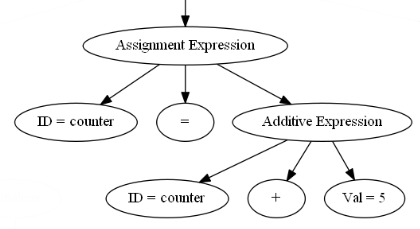
\includegraphics[width=0.6\linewidth]{unfolded_addition}
	\caption{An Assignment Expression with counter addition as value}
	\label{fig:unfolded_addition}
\end{figure}

However, the context-sensitive reduction will be able to reduce the earlier specified example to the automaton in Figure \ref{fig:folded_addition}. This automaton will be acceptable, as this is a direct use of an allowed operation.

\begin{figure}[h]
	\centering
	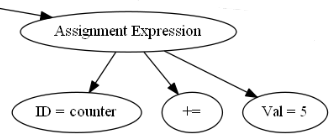
\includegraphics[width=0.5\linewidth]{folded_addition}
	\caption{An Assignment Expression with constant as value}
	\label{fig:folded_addition}
\end{figure}

\subsection{Abstract syntax tree validation}
The fourth loop will iterate over the abstract syntax tree resulting from the previous step, and while doing so, it will evaluate the nodes that occur and the context in which they occur.

The majority of the node evaluation is represented in a list of unsupported nodes. Most of these nodes are head nodes for certain kinds of expressions which will never be supported.

\begin{align*}
	unsupported = \left\{ \begin{array}{l}
		Multiplication\ Expression, sizeof, \_Alignof, \\
		\&, *, -, +, ., ->, !, ~, Cast\ Expression, \\
		Shift\ Expression, Bitwise\ And\ Expression, \\
		Bitwise\ Or\ Expression, Bitwise\ Xor\ Expression, \\
		*=, /=, \%=, <<=, >>=, \&=, ^=, |=, \\
		Logical\ And\ Expression, Logical\ Or\ Expression, \\
		Additive\ Expression
	\end{array} \right\}
\end{align*}

Whenever we encounter a node part of the $unsupported$ set, the current situation will be inspected. For example, if a \textit{Multiplication Expression} node occurs, inside a subtree of an \textit{Assignment Expression} node where an assignment to a counter was specified, we know that we are in an invalid state, as counters can only be updated via assignments, additions or subtractions. 

The same logic holds for subtrees of conditional expressions. In case we have a conditional expression where the subtree contains a \textit{Bitwise And Expression} node, we know that this is an invalid state, as constant conditions have already been folded in the previous step, this must mean that there is a counter in the condition, but counter comparisons are not allowed to contain and statements.

Furthermore, all variable usage will be tracked. We will allow multiple counters to exist, as long as we can substitute one general counter without having any conflicts, in other words, there cannot be any overlap between counter usages. This is simply tracked by tracking the nodes in which the counter variables occur, with the exception of when they occur within conditional scopes. If this is the case, their first usage is set to the first line of the scope, so that overlap does occur when a different counter is used for the condition of the scope. 

Finally, the initial value will be tracked. In case there is a declaration with an initial value, this value will be chosen, otherwise it will be set to 0, which is the default integer value in C. This initial value allows us to skip over declarations in the generator. We can simply set the counter value to the initial value of the used counter at that point in time, just before its first usage.

Another aspect that will be tested, is the function definition which can only have integer parameters. If this not the case, an error status will be added.

These conditions will all be tracked separately for each function. Whenever the status list is empty at the end of the evaluation, we assume that no issues occurred, and we say that the function satisfies the requirements, if there are any issues, no counter automaton will be generated, and the errors will be printed to the terminal.

Important to note is that there is no regard for global statements. These are considered to be variable and undetermined. It could be that they can perfectly be used as counters, and that they will never be altered by other functions, but it is impossible to determine this efficiently. Therefore, a counter must be declared within the function scope.\\
\\
\noindent
\textbf{Validation example}\\
When we go back to the earlier mentioned segment of code, given in Listing \ref{lst:ready to eval}, we obtain the automaton displayed in Figure \ref{fig:divide_cleaned}.

\begin{lstlisting}[style=CStyle, caption={Example of a ready to evaluate function}, label={lst:ready to eval}]
bool divide(int p, int n){
	int counter = p;
	
	while(counter > 0){
		counter -= n;
	}
	
	if(counter == 0){
		return true;
	}
	return false;
}
\end{lstlisting}

\begin{landscape}
	\vspace*{\fill}
	\begin{figure}[h]
		\centering
		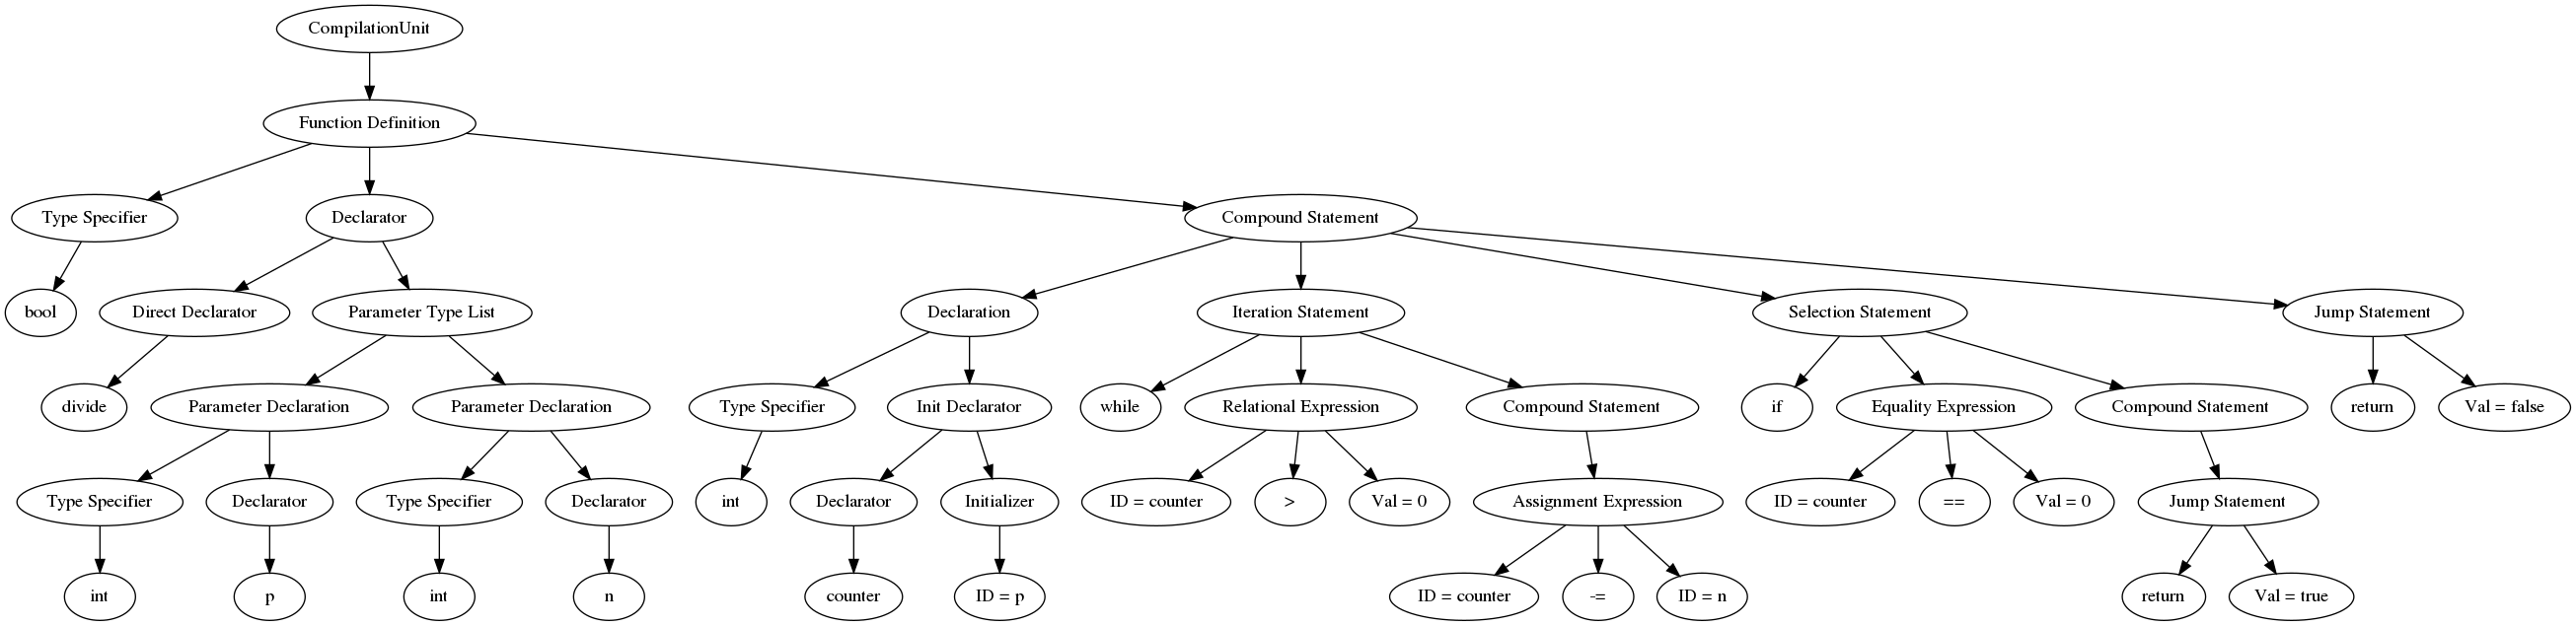
\includegraphics[width=\linewidth]{divide_cleaned}
		\caption{The cleaned Abstract Syntax Tree for the divide function}
		\label{fig:divide_cleaned}
	\end{figure}
	\vspace*{\fill}
\end{landscape}

We can immediately see that the function conforms to the required function definition, as the parameters are of type int, which can be seen from the parameters defined underneath the \textit{Parameter Type List} node.

From the cleaner we know which variables are counters, and we can see that the first declaration is a counter, but we will skip the declaration, as we know the value which is stored in the initial value, the initialization will happen before the first operation on the counter occurs. 

Next, we encounter the \textit{Iteration statement}, for which we will check the condition with the constrained conditional variable enabled. With this variable enabled, we can simply continue traversing the nodes, and in case there are any unsupported nodes, the corresponding error would automatically be generated. However, there will be no corresponding nodes, so we will leave the \textit{Relational Expression} without any error statuses, and we will disable the constrained conditional variable. 

Next we will enter the \textit{Compound Statement}, which symbolizes the inner scope of the iteration statement. We will encounter an \textit{Assignment Expression} with a variable that we know is a counter, we will therefore enable the counter assignment variable, while traversing the children of this node. No invalid nodes will appear, and we will disable the counter assignment variable when leaving the \textit{Assignment Expression} node. 

The selection statement will be evaluated in the exact same manner as the Iteration Statement was evaluated, and as the jump statement holds no special operations, we can conclude that this function satisfies the requirements for continuous one counter automaton generation.

\subsection{Counter automaton generation}
\label{sec:generation}
The final step of the conversion will be the counter generation itself. In this loop, there will be no more regards to possible invalid statements. At this point we assume everything to be known, and we can therefore simplify our analysis. Recall that the following list is the collection of allowed labels for the counter automaton.
\[
op = \{+c, -c, +p, -p, \leq c, =c, \geq c, \leq p, =p, \geq p: c \in \mathbb{N}, p \in P\} \cup \{\wedge\}
\]
This allows us to just check the head nodes related to such expressions.

\subsubsection{Functions}
First of all, we need the notion of the \textit{Function Definition} statements. The generator will generate a counter automaton for each function, and needs to know when these start.

\subsubsection{Assignments}
Other than functions, we will also need to know when assignments to counters occur, so that we can add the proper transition labels. We only need to check whether or not we are assigning to a counter, if so, we read the operation used, and the variable that gets assigned. Valid counter assignments need to be of the form \textit{c op x} where $c$ is the counter, $op \in $ \textit{\{=, +=, -=\}} and $x \in P \lor x \in \mathbb{N}$. 

As mentioned earlier, assignments are not in the set of operations, but they can be represented using the operators displayed earlier, as can be seen in Figure \ref{fig:counter_assignment}. This can be done by using a reset operation, where we first check whether or not the counter is smaller or equal to the desired value. If so, it is either already satisfied, in which case we can just carry on, or it is smaller than the desired value, for which we will add a self loop with $+1$ as a label, so that we will eventually reach the desired value. 
\begin{figure}[h]
	\centering
	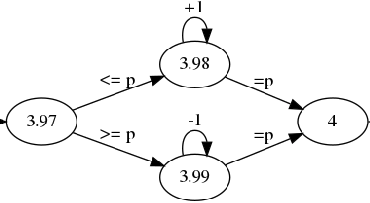
\includegraphics[width=0.48\linewidth]{counter_assignment}
	\caption{Assignment of a value p to a counter}
	\label{fig:counter_assignment}
\end{figure}

The same thing can be done when the counter is larger or equal to the desired value, if so, it is either already satisfied, in which case we can just carry on, or it is larger than the desired value, at which point we will decrement the counter with a self loop of -1, until the condition is satisfied.

An important thing to remark, is that we are not interested in general properties of runs for these automata. We are interested in the possibility of reachability or in other words, the existence of one path that will take us to a given node. In the given example, there is a path where we would remain in node 3.98 indefinitely but since there is at least one path that would take us to node 4, node 4 is still considered reachable.

\subsubsection{Inequality conditions}
\label{sec:inequality}
Another statement we will need to support, are inequality conditions. If we want our conditional statements to be properly functioning, we will need to be able to generate opposing conditions, but the opposing condition of the equality condition, is the inequality condition, which we can not directly model using the given operations.

The following code segment in Listing \ref{lst:equality} makes use of an if statement which has an equality condition in it.

\begin{lstlisting}[style=CStyle, caption={Example of C code containing an equality condition}, label={lst:equality}]
bool is_ten(int c){
	if(c == 10){
		return true;
	}

	return false;
}
\end{lstlisting}

When looking at part of a simplified counter automaton in Figure \ref{fig:inequality_expression}, we will notice the transitions going from the \textit{start\_if} node, towards the \textit{end\_if} node. There will not be an \textit{else} node, as there is no \textit{else if} or \textit{else} statement.

\begin{figure}[h]
	\centering
	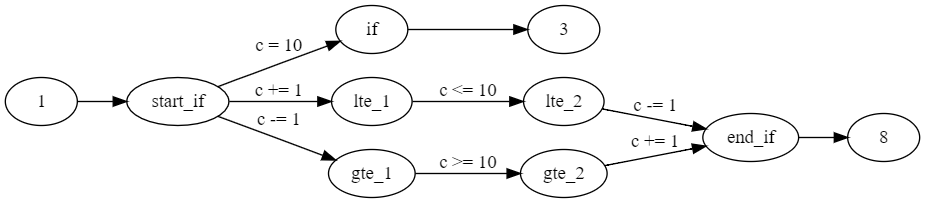
\includegraphics[width=\linewidth]{inequality_expression}
	\caption{Example of an inequality expression}
	\label{fig:inequality_expression}
\end{figure}

The first path follows the \textit{lte} nodes, which starts with \textit{c += 1} followed by \textit{c \textless =10}, followed by \textit{c -= 1}, which results in the same expression as saying the original counter is strictly smaller than 10. The final \textit{c -= 1} is there to reset the counter, so that the counter is back to what it originally was. 

The second path follows the \textit{gte} nodes, with the first transition being \textit{c -= 1}, followed by \textit{c \textgreater =10}, followed by \textit{c += 1}. This chain states that the counter must be strictly greater than 10.

If either of these can be taken, we can state that the counter must be different to the compared value (in this case 10), as these both express a strict inequality. 

\subsubsection{Less than and greater than}
\label{sec:strict}
The final addition to the set of supported statements, are the \textit{less than} and \textit{greater than} expressions. These are needed to model the opposing conditions to greater than or equal and less than or equal respectively.

\begin{lstlisting}[style=CStyle, caption={Example of a code segment using less than and less than or equal conditions}, label={lst:less than}]
bool is_ten(int c){
	if(c <= 10){
		if(c < 10){
			return false;
		}
		return true;
	}
	return false;
}
\end{lstlisting}

The code segment in Listing \ref{lst:less than} models both a less than or equal condition and a less than condition. The first condition will need to be opposed with a strictly greater than condition, and the second one with a greater than or equal condition.

\begin{figure}[h]
	\centering
	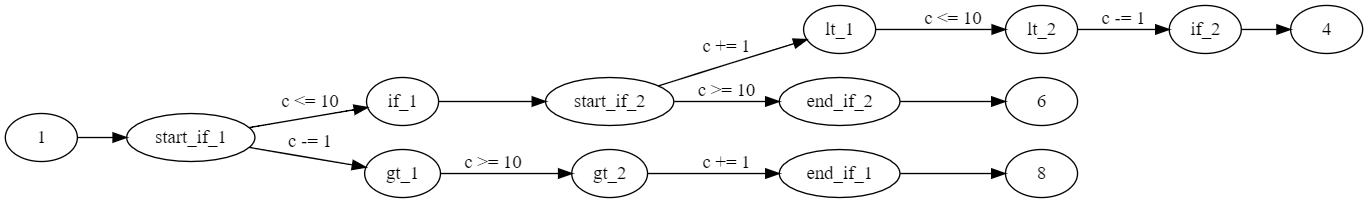
\includegraphics[width=\linewidth]{less_than_greater_than}
	\caption{Example of a less than expression and a greater than expression}
	\label{fig:less_than_greater_than}
\end{figure}

A simplified version of the counter automaton of this function can be seen in Figure \ref{fig:less_than_greater_than}. This automaton has \textit{start\_if\_1} as the start of the outer if and it has \textit{if\_1} and \textit{end\_if\_1} as respective if and end nodes. The inner if has \textit{start\_if\_2} as the start node, \textit{if\_2} as the start of the if segment, and \textit{end\_if\_2} as the end node.

The strict greater than condition, originating from node \textit{start\_if\_1} and ending in node \textit{end\_if\_1}, consists of 3 different transitions. The first transitions \textit{c -= 1} and \textit{c \textgreater =10}, test if the counter is strictly greater. The third transition \textit{c += 1} is there to make sure that the counter goes back to its original value.

The strict less than condition, originating from node \textit{start\_if\_2} and ending in node \textit{if\_2}, consists of \textit{c += 1} and \textit{c \textless =a} as their first two transitions, which can only be satisfied in case the counter is strictly less than a. The final condition \textit{c -= 1} is there to make sure the counter goes back to its original value.

\subsubsection{Iteration statements}
We will also need the notion of iteration statements, which needs 5 additional special nodes to fully support it's functionality. The first node will be the \textit{start of the loop}. The second node is the \textit{pre node} which symbolizes the state after the precondition of the for loop has been evaluated. Next we need \textit{start of the inner segment} to signify the start of the inner segment. This node will be reached by a transition with the condition as a label. 

After this node the inner segment will follow, and it will be finalized with the \textit{stop inner segment} node, in case this one is needed. This stop node will symbolize the state after the post expression of the for loop has been evaluated, after this node, a transition will occur to the pre node, to re-evaluate the loop condition.

Finally, one more node is needed, and this node will symbolize the \textit{end of the loop}. This node will always be the last node that gets generated, so that any nodes generated beyond this point will start from this point.

Consider the segment of code in Listing \ref{lst:itteration} for which the code conversion will result in the automaton in Figure \ref{fig:test_counter_automaton}.
\begin{lstlisting}[style=CStyle, caption={Example of an itteration statement}, label={lst:itteration}]
bool test(int c){
	for(c = 0; c < 5; c ++){
		continue;
	}
	return true;
}
\end{lstlisting}

\begin{figure}[h]
	\centering
	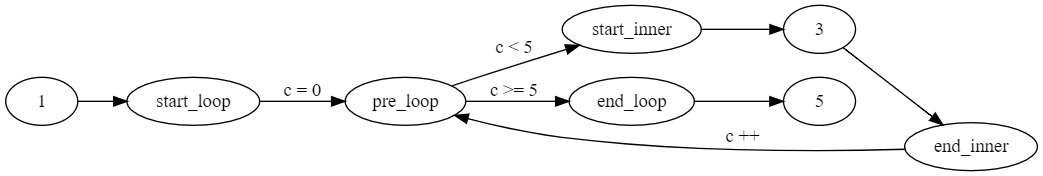
\includegraphics[width=0.95\linewidth]{test_counter_automaton}
	\caption{Example of an Iteration Statement}
	\label{fig:test_counter_automaton}
\end{figure}

\subsubsection{If statements}
\label{sec:if}
Another important construct are the if statements. These statements will, just as the iteration statements did, require additional nodes to be able to be modelled. If statements require a total of 4 nodes to be modelled.

First of all, we need a $start\ if$ node, from which the conditions will start. The $if$ and $else$ nodes will be used to signify the start of the if and else segment (if present). Independent of the presence of an $else$ node the if configuration will always end in an $end\ if$ node from which point the automaton will carry on to the next line of code.

\begin{lstlisting}[style=CStyle, caption={Example if statements}, label={lst:if}]
bool test2(int c){
	if(c == 1){
		printf("The counter is equal to 1.");
	}
	else if(c == 2){
		printf("The counter is equal to 2.");
	}
	return true;
}
\end{lstlisting}

Consider the function in Listing \ref{lst:if}. The program will return a more in depth version of the simplified counter automaton displayed in Figure \ref{fig:test2_counter_automaton}. The first if statement will start from $start\_if\_1$, and end at $end\_if\_1$, the else if will start from $start\_if\_2$, and end at $end\_if\_2$.

\begin{figure}[h]
	\centering
	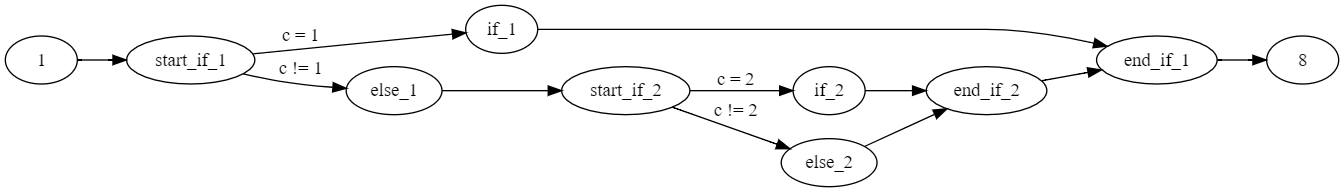
\includegraphics[width=\linewidth]{test2_counter_automaton}
	\caption{Example of if statements}
	\label{fig:test2_counter_automaton}
\end{figure}

\subsubsection{Switch statements}
A second conditional statement that exists in C, is a \textit{switch statement}. This statement allows a variable to be compared against multiple values. What is special about the switch statements, is that if matched with one case, the code of all consequential cases will also be executed, until the end of the switch, or until a jump occurs.

Consider the code snippet in Listing \ref{lst:switch}. In this case, a variable \textit{a} will be compared with multiple values, and depending on the matched case, a number of prints will occur.

\begin{lstlisting}[style=CStyle, caption={Example of a switch statement}, label={lst:switch}]
bool test(int a){
	switch(a){
		case 3:
			printf("The parameter is greater than 2.");
		case 2:
			printf("The parameter is greater than 1.");
		default:
			printf("The parameter value is %d", a);
	}
	return true;
}
\end{lstlisting}

To generate a counter automaton for a switch statement, we will start by generating a chain for the statements in the cases. This is represented by the chain starting from \textit{start\_switch}, all the way to \textit{default}, in Figure \ref{fig:counter_switch}.

After the initial node we need to add the conditional branches that correspond to the different cases. A first branch originates from \textit{start\_switch}, and can either go to \textit{case\_3} in case the counter is equal to 3, or to \textit{not\_case\_3} in case the counter is not.

There is a second branch from \textit{not\_case\_3} where we can either go to \textit{case\_2} in case the counter is equal to 2, or to \textit{not\_case\_2} in case the counter is not. Finally, from \textit{not\_case\_2} we will always go to the \textit{default} node.

\begin{figure}[h]
	\centering
	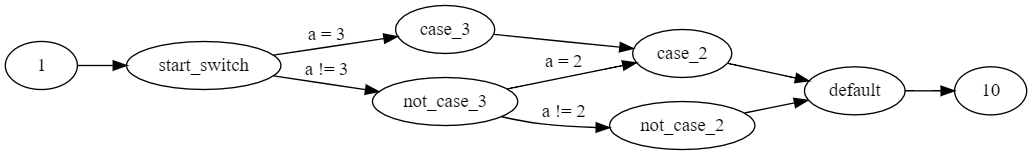
\includegraphics[width=\linewidth]{counter_switch}
	\caption{Example of a switch statement}
	\label{fig:counter_switch}
\end{figure}

\subsubsection{Counter initialization}
The counters do not get initialized at the point that they got declared within the code. This is a simple improvement that helps to reduce the number of counters. Consider the code segment in Listing \ref{lst:two counters}, in which two different counters are used.

\begin{lstlisting}[style=CStyle, caption={Example of a function with two non-overlapping counters}, label={lst:two counters}]
bool two_counters(){
	int c = 0;
	int c2 = 0;
	if(c == 2){
		return false;
	}
	else if(c2 == 2){
		return false;
	}
	return true;
}
\end{lstlisting}
The first counter will be initialized just before the if statement gets used. The second counter will not be initialized at that point, but will only be initialized just before the second if statement gets used. This means that the program will in fact be able to support the given code segment, even though it has two different counters.

\subsubsection{Final overview}
To give an in depth overview of how the conversion works, we will transform the following code snippet given in Listing \ref{lst:final overview} into a counter automaton. This code consists of multiple if statements, as well as a loop, it makes use of a single counter value, being \textit{counter}, and two parameters. The loop and the final \textit{if} both use inequality expressions, which are representable in a counter automaton, as was described earlier. The first two \textit{ifs} make use of relational expressions with the less than and greater than operators, which are also representable within a counter automaton. The counter is only  using additions or subtractions with parameters and none of these parameters will ever be modified, which also conforms to the requirements. Finally, this function has only integer parameters which makes us conclude that this entire function is representable in a counter automaton.
\newpage

\begin{lstlisting}[style=CStyle, caption={Example of a more complex function suitable for conversion}, label={lst:final overview}]
bool gcm(int a, int b){
	int counter = a;
	counter -= b;
	int i1 = 1;
	int i2 = 1;
	while(counter != 0){
		if(counter > 0){
			counter -= b;
			i2 += 1;
		}
		else if(counter < 0){
			counter += a;
			i1 += 1;
		}
		if(counter == 0){
			printf("the greatest multiple is equal to ");
			printf("%d * %d = %d * %d = %d.", i1, a, i2, b, i1*a);
		}
	}
	return true;
}
\end{lstlisting}

The first line is the function definition, this will just be converted to a node with label 1, representing the first line. Since this is the first node added to the counter automaton, it will also be denoted as being the initial node, as can be seen in Figure \ref{fig:final_overview_1}.

\begin{figure}[h]
	\centering
	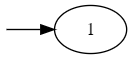
\includegraphics[width=0.2\linewidth]{final_overview_1}
	\caption{First node in the counter automaton}
	\label{fig:final_overview_1}
\end{figure}

The second line is of interest to the counter machine, as it is a counter modification. However it will not directly generate any special counter automaton configuration, as declarations of counters are only displayed as soon as a counter is actually used or modified. Since nothing special is generated, it will simply generate a new node representing the current line (being 2), with a transition coming from the last added node before this one, as displayed in Figure \ref{fig:final_overview_2}.

\begin{figure}[h]
	\centering
	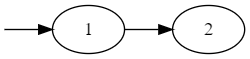
\includegraphics[width=0.4\linewidth]{final_overview_2}
	\caption{Automaton corresponding to the second line of \textit{gcm}}
	\label{fig:final_overview_2}
\end{figure}

The third line is an actual modification to the counter, so before we generate any additional nodes regarding the operation specified on this line, we need to add the counter initialization as a \textit{pre} statement for this line. This is represented in the tool by decrementing the current line in steps of 0.01. An assignment operation requires three additional nodes, so we will make use of the nodes 2.97, 2.98 and 2.99 to model the assignment functionality, as visualised in Figure \ref{fig:final_overview_3}.

\begin{figure}[h]
	\centering
	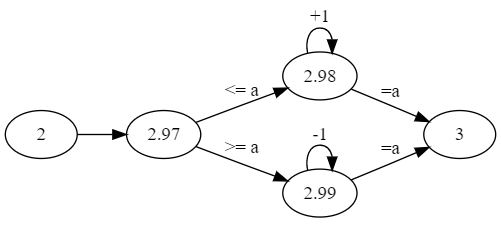
\includegraphics[width=0.7\linewidth]{final_overview_3}
	\caption{Counter automaton modelling the initial assignment of the counter}
	\label{fig:final_overview_3}
\end{figure}

The actual operation specified on line three, is a subtraction of the counter by the parameter b, as is modelled in the sub counter automaton in Figure \ref{fig:final_overview_4}.

\begin{figure}[h]
	\centering
	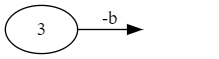
\includegraphics[width=0.35\linewidth]{final_overview_4}
	\caption{Counter automaton modelling the operation on line two}
	\label{fig:final_overview_4}
\end{figure}

Line four and five are both statements that are not of relevance to the counter, and will therefore be simply represented as a sequential chain following from the last added node, being node 3, as can be seen in Figure \ref{fig:final_overview_5}.

\begin{figure}[h]
	\centering
	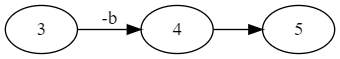
\includegraphics[width=0.5\linewidth]{final_overview_5}
	\caption{Counter automaton resulting from line four and five}
	\label{fig:final_overview_5}
\end{figure}

The sixth line defines a while loop. This requires us to add several nodes that are all related to the statement on line six. The tool will symbolise this by incrementing the current line in steps of 0.01. So 4.01 is a node that is used to help model a statement on line four.

First we need two nodes, one symbolising the start of the inner branch, modelled by the node with label 6.02, and one the symbolise the end of the loop, modelled by the node with label 6.01.

The loop ends as soon as the while condition no longer holds, and therefore the transition from start node, 6, to the end of the loop, 6.01 is a condition checking whether or not the condition of the while loop no longer holds, in this case this condition is represented as equality to zero, being the opposite condition to inequality to zero. 

The loop continues as long as the condition holds, which is modelled by the sequence going from the start node, 6.01, to the start of the inner loop, being 6.02. This configuration models an inequality to zero expression, as described in Section \ref{sec:inequality} \nameref{sec:inequality}.

\begin{figure}[h]
	\centering
	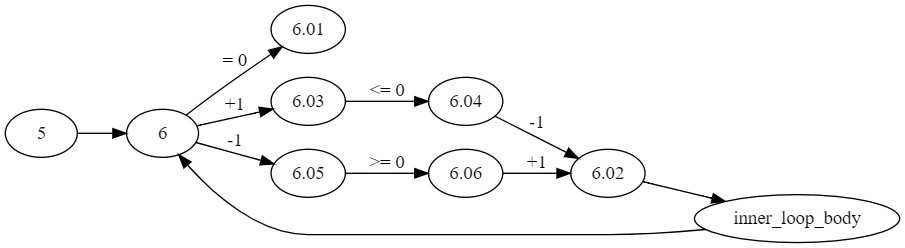
\includegraphics[width=\linewidth]{final_overview_6}
	\caption{Counter automaton resulting from line six}
	\label{fig:final_overview_6}
\end{figure}

Lines seven until ten define the first selection statement. Selection statements require, as referenced in Section \ref{sec:if} \nameref{sec:if}, three additional nodes to fully model the needed implementation.

The start of the selection statement, is modelled by the node with label 7. From this node, there is a transition going to the node with label 7.03, which symbolises the else branch, and therefore the transition to this node symbolises all counter values for which the if condition would not hold, which in this case are all counters smaller than or equal to zero.

The second transition originating from the start of the selection statement symbolises the cases where the counter satisfies the selection condition. The node 7.01 symbolises the start of the inner body of the if statement. The chain of transitions starting from 7 and going to node 7.01 model strict greater than, as is explained in Section \ref{sec:strict} \nameref{sec:strict}.

Finally, there is the \textit{end of if statement} node, being node 7.02. This node symbolises the end of all branches, so if there were any \textit{else} branches, they will also end in this node.

The inner body is simple and does not need any complex structures to be added. The statement on line 8 will result in a transition originating from node 8 with label $-= b$. The statement on line 9 has no effect on the counter, and will just be modelled with an empty transition.

\begin{figure}[h]
	\centering
	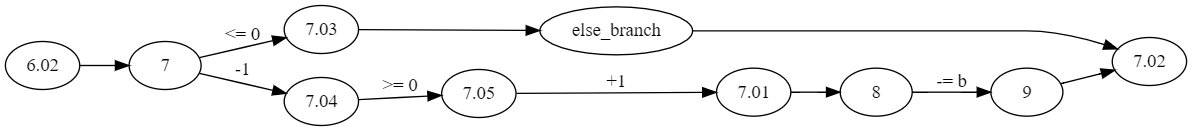
\includegraphics[width=\linewidth]{final_overview_7}
	\caption{Counter automaton resulting from line seven up until line ten}
	\label{fig:final_overview_7}
\end{figure}

The eleventh until fourteenth line models the \textit{else} branch of the previous selection statement. This statement follows the same design principles as the previous selection statement did, and will be inserted in the previous counter automaton, in the place where the current \textit{else\_branch} label is, as can be seen in Figure \ref{fig:final_overview_8}. Note that there is no \textit{else} branch, which was not generated as there are not other \textit{else if} or \textit{else} statements in the code.

\begin{figure}[h]
	\centering
	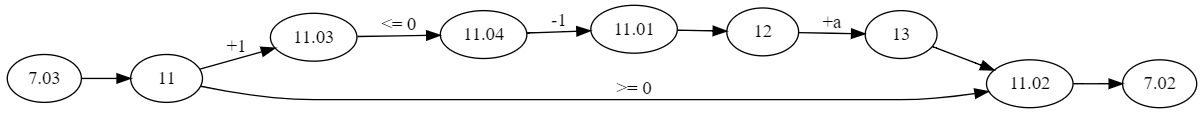
\includegraphics[width=\linewidth]{final_overview_8}
	\caption{Counter automaton resulting from line eleven up until line fourteen}
	\label{fig:final_overview_8}
\end{figure}

The final selection statement can be found on line fifteen until line eighteen. This statement includes nothing new, and will simply follow the earlier mentioned specification. This selection statement will end with a transition going from the end of the selection, being the node with label 15.02, to the start of the earlier mentioned while statement, being the node with label 6, as can be seen in Figure \ref{fig:final_overview_9}.

\begin{figure}[h]
	\centering
	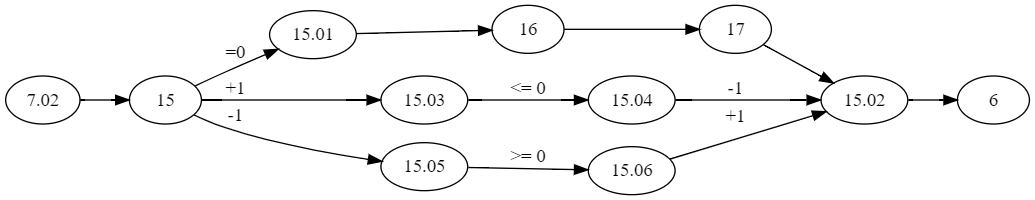
\includegraphics[width=\linewidth]{final_overview_9}
	\caption{Counter automaton resulting from line fifteen up until line eighteen}
	\label{fig:final_overview_9}
\end{figure}

After this, all that remains is the return on line twenty. This return will simply follow after node 6.01 from the while configuration specified earlier. After a return, no nodes will be generated no matter what the kind of these statements is.

\begin{figure}[h]
	\centering
	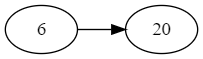
\includegraphics[width=0.35\linewidth]{final_overview_10}
	\caption{Counter automaton modelling the return on line twenty}
	\label{fig:final_overview_10}
\end{figure}

The complete overview of the counter automaton can be seen in Figure \ref{fig:final_overview_11}. This is a completely correct counter automaton that is suitable for reachability analysis.

\subsection{Automaton specification format}
\label{sec:automaton input}
For the approach described within this paper, the dot language part of Graphviz\cite{10.1007/3-540-45848-4_57} was assumed to be used to represent all automata textually. This language is a very versatile and easily understandable format in which automata can be defined. It was also used as the output language in the preceding research which automatically made it the most interesting format to support. No other formats were considered as the conversion from a textual representation to an instance of the \textit{Automaton} class is not considered to be the core of the research. The logic used for the dot language is furthermore identical to the logic that would need to be applied to read any other automaton specification, with the only difference lying in the language specific aspects of the specification.

\begin{landscape}
	\begin{figure}
		\centering
		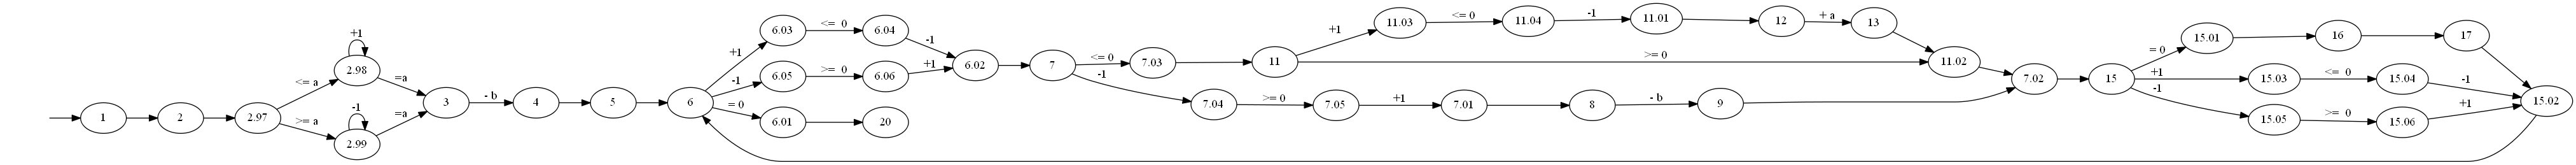
\includegraphics[width=\linewidth]{final_overview_11}
		\caption{Overview of the final resulting counter automaton}
		\label{fig:final_overview_11}
	\end{figure}
\end{landscape}

\subsubsection{Edge transformation}
Edges are represented within the dot language by a single line per edge using the format specified below. The \textit{origin} and \textit{end} tokens specify the start and end node of the transition. The square brackets encapsulate optional arguments, of which the label and xlabel arguments matter most, as either can be used to specify the label of the transition, and thereby the operation that we want to have attached to the edge. 

\begin{gather*}
	\textless origin \textgreater \rightarrow \textless end\textgreater [label=\textless label\textgreater, xlabel=\textless label\textgreater, ...]
\end{gather*}

This configuration can easily be converted into edge instances, but the labels can still represent several things. To allow any possible automaton specification, we will simply filter the labels using a regex for operations and labels. If it does not match, we assume the label to be an actual name label, if it does match, the label is perceived as a mathematical formula and it will be registered as such. 

To closely match the specification of the theoretical proof on which this approach is based \cite{blondin2021continuous}, we require edges to only contain operations and not conditions. In case an edge is encountered with a condition as a label, this will be resolved by introducing a new node, \textit{inbetween}, to which this condition will be added. This node will be added as an intermediary step and the condition label will be attached to this node. By ensuring that this node will only have one incoming edge and one outgoing edge we preserve the fact that the condition must hold in case one desires to from from the \textit{origin} node to the \textit{end} node. 

Below in Figure \ref{fig:edgetransformlabel} is an example of an edge which does not correspond to the assumptions made within the original paper as the edge between \textit{q0} and \textit{q1} has a conditional label. This is resolved in the image on the right by introducing \textit{\_0} without losing the original meaning of the edge in the first image.

\begin{figure}[h]%
	\centering
	\subfloat{
		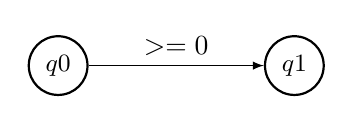
\begin{tikzpicture}[auto, >=latex, node distance = 1 cm]
		\tikzstyle{round} = [thick, draw=black, circle, font=\small]
		\tikzstyle{invis} = [draw=none, font=\small]
		
		\node[round] 	at (0, 0) 		(q0) 	{$q0$};
		\node[round] 	at (3, 0)		(q1) 	{$q1$};
		
		\path[->]
		(q0)	edge	node {$>= 0$}	(q1);
		\end{tikzpicture}
	}
	\qquad
	\subfloat{
		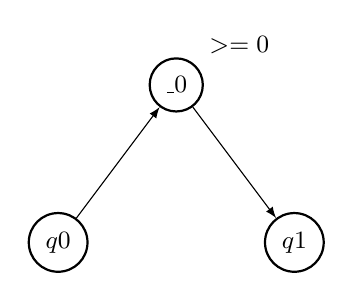
\begin{tikzpicture}[auto, >=latex, node distance = 1 cm]
		\tikzstyle{round} = [thick, draw=black, circle, font=\small]
		\tikzstyle{invis} = [draw=none, font=\small]
		
		\node[round] 	at (0, 0) 		(q0) 	{$q0$};
		\node[round] 	at (3, 0)		(q1) 	{$q1$};
		\node[invis]	at (2.3, 2.5)		(q3)	{$>=0$};
		\node[round] 	at (1.5, 2) 	(q4) 	{$\_0$};
		
		\path[->]
		(q0)	edge	node {$ $}	(q4)
		(q4)	edge	node {$ $}	(q1);
		\end{tikzpicture}
	}
	\caption{Transformation of an edge with a conditional label}
	\label{fig:edgetransformlabel}
\end{figure}

\subsubsection{Node transformation}
Nodes do not require to be specified using a separate node specification rule, and will simply be generated in case they are used within an edge. Node specifications function specifically for the cases in which additional attributes need to be added to nodes. To support operations as well as general labels, the only two attributes which will be tracked from node specification are the \textit{label} and \textit{xlabel} arguments. These labels will be matched with regexes specifying the supported formats for operations and conditions. In case the label does not match either, it is still tracked as regular node labels are still relevant for reachability reporting. For the approach discussed within this paper the node labels represent the code line from which they were generated and are therefore needed to analyse code line reachability. All node specifications will follow the format given below where the square bracket can contain a number of optional arguments.

\begin{gather*}
\textless node \textgreater [label=\textless label\textgreater, xlabel=\textless label\textgreater, ...]
\end{gather*}

To match the specification of the theoretical approach specified by Michael Blondin et Al. \cite{blondin2021continuous}, nodes can only contain conditions and not operations. In case a node \textit{origin} is found that has an operation as its label we introduce a new node \textit{inbetween}. By connecting a new edge from the \textit{origin} node to the \textit{inbetween} node we can add the label that was originally attached to \textit{origin} to the new edge. To ensure that the automaton does not lose any meaning we will then move every edge that would normally go out from \textit{origin} to \textit{inbetween}.

In Figure \ref{fig:nodetransformlabel} below, an example can be seen where node \textit{q1} is not conformant to the original specification. This is resolved by introducing \textit{\_0} from which the edge that was originally going from \textit{q1} to \textit{q2} gets reattached.

\begin{figure}[h]%
	\centering
	\subfloat{
		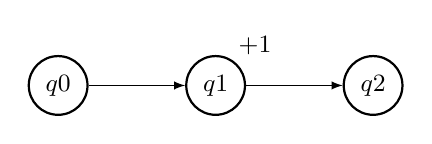
\begin{tikzpicture}[auto, >=latex, node distance = 1 cm]
		\tikzstyle{round} = [thick, draw=black, circle, font=\small]
		\tikzstyle{invis} = [draw=none, font=\small]
		
		\node[round] 	at (0, 0) 		(q0) 	{$q0$};
		\node[round] 	at (2, 0)		(q1) 	{$q1$};
		\node[invis]	at (2.5, 0.5)	(q3)	{$+1$};
		\node[round] 	at (4, 0) 		(q2) 	{$q2$};
		
		\path[->]
		(q0)	edge	node {$ $}	(q1)
		(q1)	edge	node {$ $}	(q2);
		\end{tikzpicture}
	}
	\qquad
	\subfloat{
		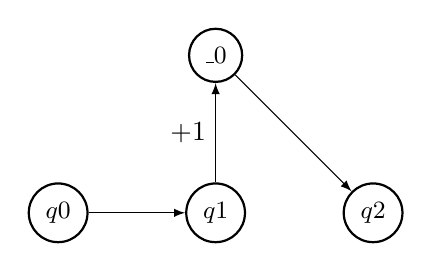
\begin{tikzpicture}[auto, >=latex, node distance = 1 cm]
		\tikzstyle{round} = [thick, draw=black, circle, font=\small]
		\tikzstyle{invis} = [draw=none, font=\small]
		
		\node[round] 	at (0, 0) 		(q0) 	{$q0$};
		\node[round] 	at (2, 0)		(q1) 	{$q1$};
		\node[round] 	at (4, 0) 		(q2) 	{$q2$};
		\node[round] 	at (2, 2) 		(q4) 	{$\_0$};
		
		\path[->]
		(q0)	edge	node {$ $}	(q1)
		(q4)	edge	node {$ $}	(q2)
		(q1)	edge	node {$+1$}	(q4);
		\end{tikzpicture}
	}
	\caption{Transformation of a node with an operational label}
	\label{fig:nodetransformlabel}
\end{figure}

\subsubsection{Initial node}
For reachability analysis to be relevant there needs to be an initial node. In automata, the initial node is often represented by a transition going from nowhere towards a single node. This is however not a built in feature within the dot language. One of the solutions to overcome this is to create a node and make it invisible, an edge can then be drawn from this invisible node to the actual initial node. Other approaches are potentially possible but were not explored. Any alternative implementations could easily be introduced instead of the considered format without interchanging any of the other components.

As a consequence of this feature invisible nodes are assumed to exist within the automaton but these are irrelevant to our analysis. Invisible nodes are by definition not relevant for reachability analysis and are therefore not considered as actual nodes.

\subsection{Reachability of non-parametric COCA}
\label{sec:reachability non parametric}
In this section we will give a description of the solution that was used to determine the reachability for non-parametric continuous one counter automata. This will be done by showing the approach that was taken, as well as an application to show its usage. This approach is a practical implementation of the theoretical approach described by Michael Blondin et al. \cite{blondin2021continuous}.

\subsubsection{Initialization}
During the initialization phase, we will instantiate all reachability intervals. The initial node will get an initial reachability interval $[i, i]$ where $i$ represents the initial counter value. This is not a fixed value, but will for the sake of this research always default to 0, simply because all integer values in most programming languages default to 0 at initialization.

All other nodes will get an empty interval assigned to them as to signify that they are initially not reachable.

\subsubsection{Interval updates}
\label{interval updates}
From the initial state, we will start doing cycles in which we update all intervals once, wherever possible. This will be done using the successor function \textit{succ} below where $R_i: Q \times Q \rightarrow 2^\mathbb{Q}$ represent the mapping function for the i-th iteration. This function is going from each transition to its corresponding counter reachability interval. The \textit{succ} function will update the interval of one transition, \textit{(p, z, q)}, to its next iteration, based upon the current configuration.

\begin{gather*}
	\hspace{-125 pt} succ_{p, q}(R_i) := \bigcup \{R_i(q, l)\,|\,(q,z,l) \in T\}\\
	\hspace{60 pt} \cup \bigcup \{(R_i(p, q) + (0, z]) \cap (q)\,|\,(p,z,q) \in T, z>0\}\\
	\hspace{60 pt} \cup \bigcup \{(R_i(p, q) + (z, 0]) \cap \tau(q)\,|\,(p,z,q) \in T, z<0\}\\
	\hspace{-20 pt} \cup \bigcup \{R_i(p, q) \cap \tau(q)\,|\,(p,0,q) \in T\}
\end{gather*}

This formula allows us to iteratively compute the next interval configuration to fully explore which states have a non empty interval. Consider the example given in Figure \ref{fig:example_succ}. We will initialise $R_0$ such that all states have empty intervals, with the exception of the first state which we will initialise to $[0, 0]$. Note that these intervals are stored per pair of final and preceding node and not per node in general. This is because this allows us to have a better tracking of which path has which effect, which will help us in later steps. In the end it suffices to know that a node is reachable, independent on the path via which it can be reached.

\begin{figure}[h]%
	\centering
	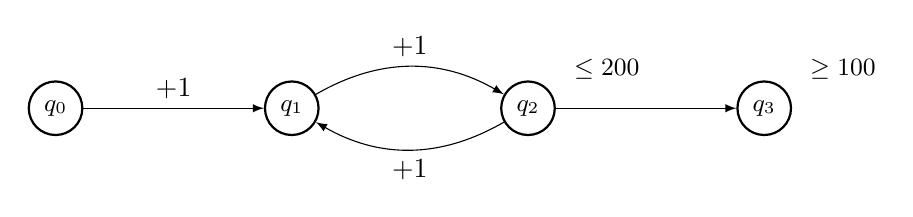
\begin{tikzpicture}[auto, >=latex, node distance = 1 cm]
		\tikzstyle{round} = [thick, draw=black, circle, font=\small]
		\tikzstyle{invis} = [draw=none, font=\small]
		\tikzstyle{arrow} = [thick,->,>=stealth]
		
		\node[round] 	at (0, 0) 		(q0) 	{$q_0$};
		\node[round] 	at (3, 0)		(q1) 	{$q_1$};
		\node[round] 	at (6, 0)		(q2) 	{$q_2$};
		\node[invis]	at (7, 0.5)		(q4)	{$\leq 200$};
		\node[round] 	at (9, 0)		(q3) 	{$q_3$};
		\node[invis]	at (10, 0.5)	(q4)	{$\geq 100$};
		
		\path[->]
			(q0) 	edge 					node 					{$+1$}	(q1)
			(q1) 	edge 	[bend left]		node	[right, above] 	{$+1$} 	(q2)
			(q2)	edge 	[bend left]		node	[right, below]	{$+1$}	(q1)
			(q2)	edge 					node					{}		(q3);
	\end{tikzpicture}
	\caption{Example of a guarded automaton on which the succ function can be applied}
	\label{fig:example_succ}
\end{figure}

\begin{table}[h]
	\begin{tabular}{ |c|c|c|c|c|c|c|c| }
		\hline
		p		& q 	& $R_0$ 		& $R_1$			& $R_2$			& $R_3$			& $R_4$ 		& $R_5$ \\
		\hline
		$q_0$	& $q_0$ & [0, 0] 		& [0, 0] 		& [0, 0] 		& [0, 0]		& [0, 0]		& [0, 0] \\
		$q_0$	& $q_1$ & $\emptyset$ 	& (0, 1]		& (0, 1] 		& (0, 1]		& (0, 1] 		& (0, 1] \\
		$q_1$	& $q_2$ & $\emptyset$ 	& $\emptyset$ 	& (0, 2] 		& (0, 2]		& (0, 4] 		& (0, 4] \\
		$q_2$	& $q_1$ & $\emptyset$ 	& $\emptyset$ 	& $\emptyset$	& (0, 3]		& (0, 3] 		& (0, 5] \\
		$q_2$	& $q_3$ & $\emptyset$ 	& $\emptyset$ 	& $\emptyset$	& $\emptyset$	& $\emptyset$	& $\emptyset$ \\
		\hline
	\end{tabular}
	\centering
	\caption{Interval configuration when acceleration is not applied}
	\label{table:table_example_succ}
\end{table}

For the first successor, we will only update for the transition going from $q_0$ to $q_1$ as this is the only transition where there is a non empty predecessor. All other transitions will both have an empty interval for the start and end nodes which will therefore trivially result in empty intervals after applying the \textit{succ} function. When we apply the \textit{succ} function on the first interval, we will get $(0, 1]$ as a resulting interval. The 0 is not included as the $(0,z]$ with $z=1$ which we will add to it does not include 0. As $q_1$ has no condition the $\tau(q_1)$ will simply be $(-\infty, \infty)$ and will therefore have no effect.

The second successor will update for the transition going from $q_1$ to $q_2$. This update will be similar to the update that happened for $q_0$ to $q_1$ in every way but the starting interval, which is now (0, 1] and will thus result in an interval of (0, 2].

Next, for the third successor, one would say that we can update both the transition going back form $q_2$ to $q_1$ and the transition going from $q_2$ to $q_3$. However, the latter is not updatable as $R_2(q_2) \cap \tau(q_3)$ will result in an empty set, considering that $\tau(q_3) = [100, \infty)$.

As can be seen in Table \ref{table:table_example_succ} a few more successors were computed and we can clearly notice that we will eventually reach an interval which will exceed the lower bound of 100 which is placed upon $q_3$. Given that the interval of $q_2$ goes up by two every other iteration it will take up to cycle 100 before the transition becomes active. Considering that this is only a small example, this is far from desired. Furthermore, given a loop that is not bounded, it is possible that a loop has no fix point at all, which means that our algorithm will evaluate indefinitely. A solution for this is loop acceleration in which we will accelerate our loop based upon the behaviour said loop shows. 

\subsubsection{Loop acceleration}
\label{sec:accel}
Unfortunately, the \textit{succ} function is not guaranteed to find the bounds in a finite number of evaluations. For example, the scenario given in Figure 23 would never converge at all. The interval of the loop between $q_1$ and $q_2$ will keep expanding indefinitely and the evaluation will therefore never stop.

To perform loop acceleration we need to consider the notion of \textit{expanding cycles}. A cycle or loop is considered to be \textit{positively expanding} if there is a path that follows a state sequence $q_i, q_{i+1}, q_{i+2}, ..., q_{n-1}, q_n$ evaluated in reachability iterations $R_0, R_{1}, R_{2}, ..., R_{k-1}, R_{k}$, where k represents the current iteration, such that:
\begin{enumerate}
	\item $q_i = q_n$
	\item $\forall j \in [i, n-1]: (p_j, z_j, q_{j+1}) \in T$
	\item $\forall j \in [i, n-1]: R_k(p_j, q_{j+1}) \ne \emptyset$
	\item $\exists (p, z, q) \in T: z > 0$
	\item $sup(R_k(q_{n-1}, q_{n})) > sup(R_{k-1}(q_{n-1}, q_n))$
\end{enumerate}

Similarly we say that a cycle is \textit{negatively expanding} if the following hold:
\begin{enumerate}
	\item $q_i = q_n$
	\item $\forall j \in [i, n-1] : (p_j, z_j, q_{j+1}) \in T$
	\item $\forall j \in [i, n-1]: R_k(p_j, q_{j+1}) \ne \emptyset$
	\item $\exists (p, z, q) \in T: z < 0$
	\item $inf(R_k(q_{n-1}, q_{n})) < inf(R_{k-1}(q_{n-1}, q_n))$
\end{enumerate}

The first condition in combination with the second condition simply implies that we require there to be an actual loop. The third condition states that we should have visited every transition at least once. In case we did not have sufficient information needed to perform the acceleration we can not know the full behaviour of the loop. We will therefore only mark loops as expanding in case we have fully discovered it. This also eliminates the potential that we are looking at loops where some of the nodes are not reachable due to node constraints present within the loop. The fourth and fifth condition are there to ensure that there is an actual expansion. If only the fifth condition holds, it implies that there was a change in supremum due to something outside of the loop, in case only the fourth condition holds but not the fifth, it implies that we have already reached the bound of the loop. In the latter case the loop will not be marked as expanding as this implies that it reached its bound after one iteration.

Given that we know whether or not a cycle is either positively or negatively expanding, we can derive which node will reach its bound first. By doing so we can move the interval to this bound and thus greatly accelerate the evaluation of said loop. By performing one more iteration throughout the loop, all bounds would be reached and no further evaluation of the before mentioned loop will be needed.

To find the node that will be the first to reach a fix point interval, we can simply consider the node for which the current reachability interval's supremum/infimum is closest to the max/min node bound given that we are either trying to accelerate upwards or downwards respectively. In the formula below $reach(q)$ represents a function denoting the set of final counter values for a state $q$ and $\underline{\tau}(q_j)$ and $\overline{\tau}(q_j)$ represent the upper and lower node bounds of node $q_j$ respectively.\\
\\
\noindent
Given a loop that is expanding positively. If the following properties evaluate to true:

\begin{itemize}
	\item $sup(R_i) > sup(R_n)$
	\item $\exists (p, z, q) \in T: z > 0$
	\item $\overline{\tau}(q_k) - v_k = min_{i\leq j \le n}\,\overline{\tau}(q_j) - v_j$
\end{itemize}
The following property will apply:
\begin{itemize}
	\item $[v_k, \overline{\tau}(q_k)] \subseteq reach(q_k)$
\end{itemize}


\noindent
Given a loop that is expanding negatively. If the following properties evaluate to true:

\begin{itemize}
	\item $inf(R_i) < inf(R_n)$
	\item $\exists (p, z, q) \in T: z < 0$
	\item $v_k - \underline{\tau}(q_k) = min_{i\leq j \le n}\,v_j - \underline{\tau}(q_j)$
\end{itemize}
The following property will apply:
\begin{itemize}
	\item $[\underline{\tau}(q_k), v_k] \subseteq reach(q_k)$
\end{itemize}

In our approach this allows us to traverse the differences between the previous iteration and the current iteration whenever we update a node that we already have an interval for. Given the example that was explored in Section \nameref{interval updates} we can see that we have a loop going from $q_1$ to $q_2$ and back. 

\begin{table}[h]
	\begin{tabular}{ |c|c|c|c|c|c|c|c| }
		\hline
		p		& q 	& $R_0$ 		& $R_1$			& $R_2$			& $R_3$			& $R_4$ 		& $R_5$ \\
		\hline
		$q_0$	& $q_0$ & [0, 0] 		& [0, 0] 		& [0, 0] 		& [0, 0]		& [0, 0]		& [0, 0] \\
		$q_0$	& $q_1$ & $\emptyset$ 	& (0, 1]		& (0, 1] 		& (0, 1]		& (0, 1] 		& (0, 1] \\
		$q_1$	& $q_2$ & $\emptyset$ 	& $\emptyset$ 	& (0, 2] 		& (0, 2]		& (0, 4] 		& (0, 4] \\
		$q_2$	& $q_1$ & $\emptyset$ 	& $\emptyset$ 	& $\emptyset$	& (0, 3]		& (0, 3] 		& (0, 5] \\
		$q_2$	& $q_3$ & $\emptyset$ 	& $\emptyset$ 	& $\emptyset$	& $\emptyset$	& $\emptyset$	& $\emptyset$ \\
		\hline
	\end{tabular}
	\centering
	\caption{Resulting interval configuration before acceleration}
	\label{table:table_example_no_acc}
\end{table}

In Table \ref{table:table_example_no_acc} we can see that in the third reachability interval, $R_2$, a counter value interval is discovered for the transition going from $q_1$ to $q_2$. In the next reachability interval the same happens for $q_2$ to $q_1$. In $R_4$ we will once again update the interval for the transition going from $q_1$ to $q_2$ which will result in all conditions for a positive expanding loop evaluating to true. This is because we have a loop of which we know that the supremum of one of the transitions just increased and we have a transition part of this loop with a strictly positive operation.

Applying our previously described steps, we will find that node $q_2$ is closest to its bound and we will therefore choose to expand the interval of the transition ending in this node, being the transition from $q_1$ to $q_2$. The result is shown in Table \ref{table:table_example_acc}.

\begin{table}[t!]
	\begin{tabular}{ |c|c|c|c|c|c|c|c| }
		\hline
		p		& q 	& $R_0$ 		& $R_1$			& $R_2$			& $R_3$			& $R_4$ 		& $R_5$ \\
		\hline
		$q_0$	& $q_0$ & [0, 0] 		& [0, 0] 		& [0, 0] 		& [0, 0]		& [0, 0]		& [0, 0] \\
		$q_0$	& $q_1$ & $\emptyset$ 	& (0, 1]		& (0, 1] 		& (0, 1]		& (0, 1] 		& (0, 1] \\
		$q_1$	& $q_2$ & $\emptyset$ 	& $\emptyset$ 	& (0, 2] 		& (0, 2]		& (0, 200] 		& (0, 200] \\
		$q_2$	& $q_1$ & $\emptyset$ 	& $\emptyset$ 	& $\emptyset$	& (0, 3]		& (0, 3] 		& (0, 201] \\
		$q_2$	& $q_3$ & $\emptyset$ 	& $\emptyset$ 	& $\emptyset$	& $\emptyset$	& $\emptyset$	& [100, 200] \\
		\hline
	\end{tabular}
	\centering
	\caption{Resulting interval configuration after acceleration}
	\label{table:table_example_acc}
\end{table}

If we do one additional iteration, we can see that we have now discovered an interval for the transition going from $q_2$ to $q_3$. We have furthermore achieved a fix point, as both $q_2$ and $q_3$ have met their bounds.

\subsubsection{Proof of termination}
The mathematical proof of termination has already been given by Michal Blondin et al. \cite{blondin2021continuous} but an intuitive proof for the algorithm will also be given here. Given that there are no loops it will trivially terminate within n evaluations, given that n is equal to the total number of nodes within the automaton. If there are loops they must either be positively expanding, negatively expanding, expanding in both directions or not expanding at all. 

\begin{figure}[b!]%
	\centering
	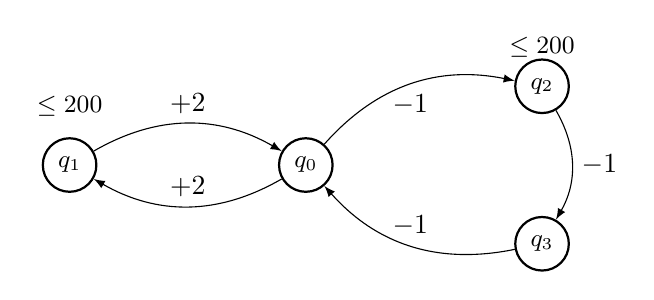
\begin{tikzpicture}[auto, >=latex, node distance = 1 cm]
		\tikzstyle{round} = [thick, draw=black, circle, font=\small]
		\tikzstyle{invis} = [draw=none, font=\small]
		\tikzstyle{arrow} = [thick,->,>=stealth]
		
		\node[round] 	at (0, 0)		(q1) 	{$q_0$};
		\node[round] 	at (-3, 0)		(q2) 	{$q_1$};
		\node[invis]	at (-3, 0.75)	(q3)	{$\leq 200$};
		\node[round] 	at (3, 1)		(q4) 	{$q_2$};
		\node[invis]	at (3, 1.5)		(q5)	{$\leq 200$};
		\node[round] 	at (3, -1)		(q6) 	{$q_3$};
		
		\path[->]
		(q1) 	edge 	[bend left]		node	[right, above] 	{$+2$} 	(q2)
		(q2)	edge 	[bend left]		node	[right, above]	{$+2$}	(q1)
		(q1) 	edge 	[bend left]		node 	[right, below]	{$-1$}	(q4)
		(q4) 	edge 	[bend left]		node	[right]		 	{$-1$} 	(q6)
		(q6)	edge 	[bend left]		node	[right, above]	{$-1$}	(q1);
	\end{tikzpicture}
	\caption{Example of an automaton in which post acceleration evaluation is needed}
	\label{fig:example_recomputation_of_bounds}
\end{figure}

In the last case the evaluation will trivially terminate as the loops will end in a fix point after their first evaluation. In the first case it will also terminate as loops can only be fully evaluated twice before reaching their fix point. One traversal is needed to discover the loop and a second to make sure that all intervals reach their fix point within said loop.

It is possible that further evaluations require bounds to be recomputed. For example, given the automaton described in Figure \ref{fig:example_recomputation_of_bounds}. In this automaton the loop between $q_0$ and $q_1$ will be expanded first. The evaluation of the second loop continues and the lower bound of $q_0$ to $q_1$ will keep on decreasing, until it eventually gets accelerated, at which moment we achieve a fix point and the evaluation stops. This will always be the case given that we can never have an infinite amount of nodes which will thus result in a finite amount of loops which all accelerate at some point. The effects of said acceleration might need a few more iterations to propagate their effect all across the automaton but once it does the evaluation will end. We can therefore conclude that the algorithm can never run indefinitely.

\subsection{Reachability of parametric COCA}
\label{sec:reachability parametric}
Throughout this section we will give an overview of how the reachability for parametric continuous one counter automata can be analysed. This will be done using the approach that was theoretically described by Michael Blondin et al. \cite{blondin2021continuous}. This paper will both give a practical approach as well as an application, intended as prove that it works in practise.

In this approach we will attempt to encode the fix-point of the \textit{succ} function defined in the previous section using first order logic which can then be implemented and solved by a SAT solver.

\subsubsection{Transition initialization}

During initialization we will start by converting all transitions that are defined within the given automaton to their equivalent equations. All transitions are represented by three variables. Two variables are used to represent the start and end point of the transition and the third will represent the operation associated with the transition. The operation will simply be an integer value as we limited our automata to only allow + and - operations. This means that an integer can fully cover every possible operation that can be performed on an edge. 

For the example given in Figure \ref{fig:example transition conversion} this would be a conversion to $(q_0, +a, q_1)$. In this resulting triple our operation is a variable which represents an integer which will be filled in by the SAT-solver.

Note that there is no need to cover conditions on edges as we resolved all inconsistencies regarding transitions with conditional labels in our automaton input phase.
\begin{figure}[t!]%
	\centering
	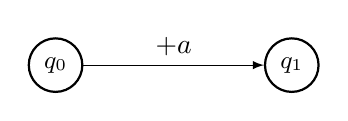
\begin{tikzpicture}[auto, >=latex, node distance = 1 cm]
		\tikzstyle{round} = [thick, draw=black, circle, font=\small]
		\tikzstyle{invis} = [draw=none, font=\small]
		\tikzstyle{arrow} = [thick,->,>=stealth]
		
		\node[round] 	at (0, 0)		(q1) 	{$q_0$};
		\node[round] 	at (3, 0)		(q2) 	{$q_1$};
		
		\path[->]
		(q1) 	edge	node	[right, above] 	{$+a$} 	(q2);
	\end{tikzpicture}
	\caption{Example of a transition before conversion}
	\label{fig:example transition conversion}
\end{figure}

\subsubsection{Node condition initialization}

Alongside the transitions we will also initialise the conditions of the nodes in which the transitions end. These are important as these decide whether or not a transition can be taken. Given that we have a transition with an operation equal to $+1$, a current counter value equal to just $0$ and an end node with a condition equal to $\le -1$. This example is visualised in Figure \ref{fig:example node condition conversion} and we can see that $q_1$ will not be reachable, given that the initial counter value is equal to 0. Each condition will be represented by two variables, one to indicate the condition type and a second to indicate the value against which it is compared. Just as for the transitions our condition value can either be constant or a variable. The condition type can have three different values, $0$ will be used to represent the $\ge$ operation, $1$ will be used to represent $\le$, 2 will represent $=$ and finally $3$ will be used in case there is no condition associated with the end node.

\begin{figure}[h]%
	\centering
	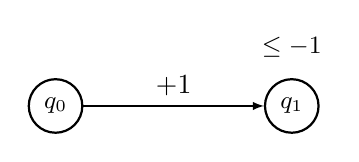
\begin{tikzpicture}[auto, >=latex, node distance = 1 cm]
		\tikzstyle{round} = [thick, draw=black, circle, font=\small]
		\tikzstyle{invis} = [draw=none, font=\small]
		\tikzstyle{arrow} = [thick,->,>=stealth]
		
		\node[round] 	at (0, 0)		(q1) 	{$q_0$};
		\node[round] 	at (3, 0)		(q2) 	{$q_1$};
		\node[invis]	at (3, 0.75)	(q3)	{$\leq -1$};
		
		\path[->]
		(q1) 	edge	node	[right, above] 	{$+1$} 	(q2);
	\end{tikzpicture}
	\caption{Example of a transition with an unsatisfiable node condition}
	\label{fig:example node condition conversion}
\end{figure}

\subsubsection{Interval encoding}

Each of the nodes will get reachability intervals assigned to it. These reachability intervals will represent a possible subset of counter values that can be reached in a given node. Using these intervals we can then decide whether or not a next transition can be taken. These intervals will also be used to derive whether or not a node is reachable.

It was proven by Michael Blondin et al. \cite{blondin2021continuous} that the number of intervals per node is bounded by $4(|Q| + 1)$ where Q is the set of all nodes. This means that we will have to generate as many intervals for each of the nodes. For these intervals we will attempt to keep as many of them empty, as to not needlessly complicate the computation.

Each interval will be represented by 4 variables. The first two variables will represent the lower and upper bound of the interval, the last two will represent whether or not these bounds are inclusive. A 0 indicates not inclusive, a 1 indicates inclusive and a 2 indicates that the bound goes until infinity. For example, an interval with just 0, $[0, 0]$ would be represented by $0, 0, 1, 1$. An interval that goes from negative infinity to 1, $(-\infty, 1]$ would be represented by $0, 1, 2, 1$ and an empty interval, $(0, 0)$ by $0, 0, 0, 0$.

Initially the start node of the automaton will have an interval equal to exactly the starting value of the counter (by default this will be 0). All other intervals of all nodes will get values according to the edges that exist within the automaton. The evolution of these intervals will be discussed in the next sections.

\subsubsection{Define the end goal}
One by one we will verify for each node whether or not it is reachable, this can be done using the condition below, where e represents the edge taken to generate any of the intervals part of the goal node. In case e is equal to -2 it signifies that no transition was taken and that the interval is empty. If e is not equal to -2 it must imply that the according interval is not empty as will be explained later.

\begin{gather*}
	\hspace{-102 pt}reachable_i = e_i \ne -2 \\
	reachable = Or(reachable_i \text{ for all i $\in$ I})
\end{gather*}

\subsubsection{msum}
The msum function is used to determine the inclusiveness of the bounds in the interval addition. The msum function is defined as:

\begin{gather*}
msum(i, j) = 2 \qquad \qquad if \; max(i,j) = 2 \\
msum(i, j) = min(i, j) \quad \qquad \quad otherwise \qquad \qquad \qquad
\end{gather*}

\subsubsection{Emptiness of intervals}
We need to be able to verify whether or not an interval is empty in order to create base cases for future operations. An interval is considered to be empty if both bounds are not inclusive and the boundary values are equal to each other as can be seen in the formulae below. 

\begin{gather*}
	x_2 = 0 \\
	x_3 = 0 \\
	x_0 = x_1
\end{gather*}

\subsubsection{Interval addition}
The addition of intervals will be split in three different cases as can be seen in the graph below. In case either operand is an empty interval the resulting interval will trivially equal the other interval. In case they are both not empty we compute the sum by taking the addition of the lower and upper bound of the X and Y intervals and the msum to compute whether or not the resulting bounds are inclusive. An overview of this can be found in Figure \ref{fig:addition}.

\begin{figure}[h]
	\centering
	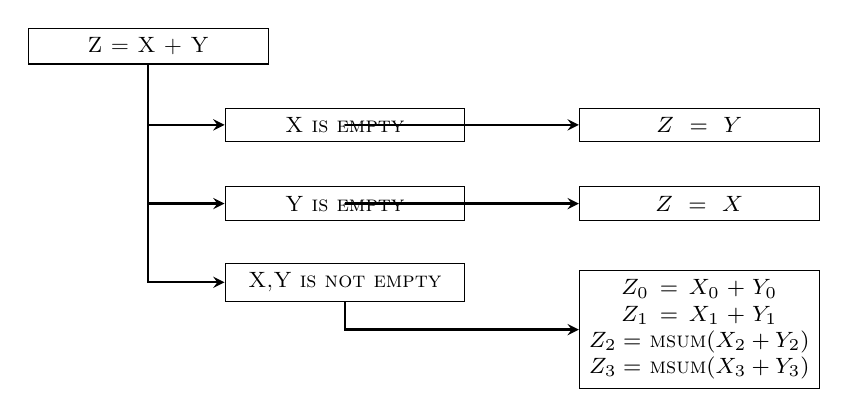
\begin{tikzpicture}[auto, >=latex, font=\footnotesize\scshape]
		\tikzstyle{small} = [draw=black, rectangle]
		\tikzstyle{center} = [draw=black, rectangle, text width=8em, align=center]
		\tikzstyle{arrow} = [thick,->,>=stealth]
		
		\node[center]	at (-0.5, 0) 	(q0) 	{Z = X + Y};
		
		\node[center]	at (2, -1) 		(q1) 	{X is empty};
		\node[center]	at (2, -2)		(q2)	{Y is empty};
		\node[center]	at (2, -3)		(q3)	{X,Y is not empty};
		
		\node[center] 	at (6.5, -1)	(q4)	{$Z = Y$};
		\node[center] 	at (6.5, -2)	(q5)	{$Z = X$};
		\node[center] 	at (6.5, -3.6)	(q6)	{$Z_0 = X_0 + Y_0$ \\
												 $Z_1 = X_1 + Y_1$ \\
												 $Z_2 =$ msum$(X_2 + Y_2)$ \\
												 $Z_3 =$ msum$(X_3 + Y_3)$};
		
		\draw [arrow] (q0) |- (q1);
		\draw [arrow] (q0) |- (q2);
		\draw [arrow] (q0) |- (q3);
		
		\draw [arrow] (q1) |- (q4);
		\draw [arrow] (q2) |- (q5);
		\draw [arrow] (q3) |- (q6);
	\end{tikzpicture}
	\caption{Overview of the interval addition operation}
	\label{fig:addition}
\end{figure}

\subsubsection{Interval overlap}
\begin{figure}[b!]
	\centering
	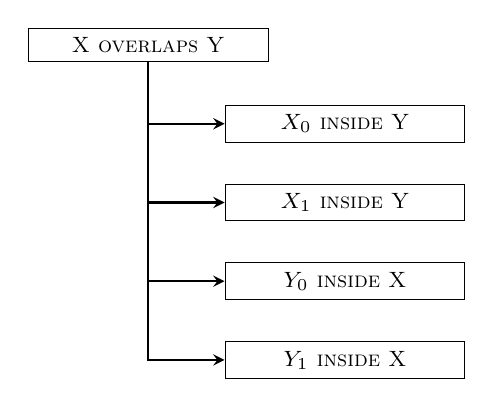
\begin{tikzpicture}[auto, >=latex, font=\footnotesize\scshape]
		\tikzstyle{small} = [draw=black, rectangle]
		\tikzstyle{center} = [draw=black, rectangle, text width=8em, align=center]
		\tikzstyle{arrow} = [thick,->,>=stealth]
		
		\node[center]	at (-0.5, 0) 	(q0) 	{X overlaps Y};
		
		\node[center]	at (2, -1)		(q3)	{$X_0$ inside Y};
		\node[center]	at (2, -2)		(q4)	{$X_1$ inside Y};
		\node[center]	at (2, -3)		(q5)	{$Y_0$ inside X};
		\node[center]	at (2, -4)		(q6)	{$Y_1$ inside X};
		
		\draw [arrow] (q0) |- (q3);
		\draw [arrow] (q0) |- (q4);
		\draw [arrow] (q0) |- (q5);
		\draw [arrow] (q0) |- (q6);
	\end{tikzpicture}
	\caption{Overview of the interval overlap operation}
	\label{fig:overlap}
\end{figure}

One important relationship between two intervals is overlap as it directly helps to simplify the generation of unions and intersections of intervals. This can be computed by verifying whether or not any of the endpoints of one interval is within the other interval. Note that it is important to specifically look at the third and fourth variable part of the interval to also consider infinite bounds. An overview of this operation can be seen in Figure \ref{fig:overlap}.

\subsubsection{Interval intersection}
The entirety of the intersection operation is visualised in Image \ref{fig:intersection}. In this image all nodes where multiple lines leave are assumed to imply $or$ operations between all end nodes. This holds with the exception of the coloured nodes where nodes of the same colour represent an $or$ operation which will then be combined in a bigger $and$.

For the intersection of intervals we will first of all consider the cases where the result is an empty vector. This can either occur when there is no overlap or when X or Y is empty. In any of these cases we can simply assign an empty vector to Z, being the resulting interval.

If this is not the case we will separately evaluate both borders of the interval. The lower border is represented by the red colour and the upper border by the blue colour within Image \ref{fig:intersection}. 

For both sides it holds that if either X or Y goes to infinity in that direction then Z will have the boundary values of the other interval. For example if X would go to infinity on the lower bound then the value of Z will be equal to the value of Y for both the lower bound value and whether or not this bound is inclusive.

\begin{figure}
	\centering
	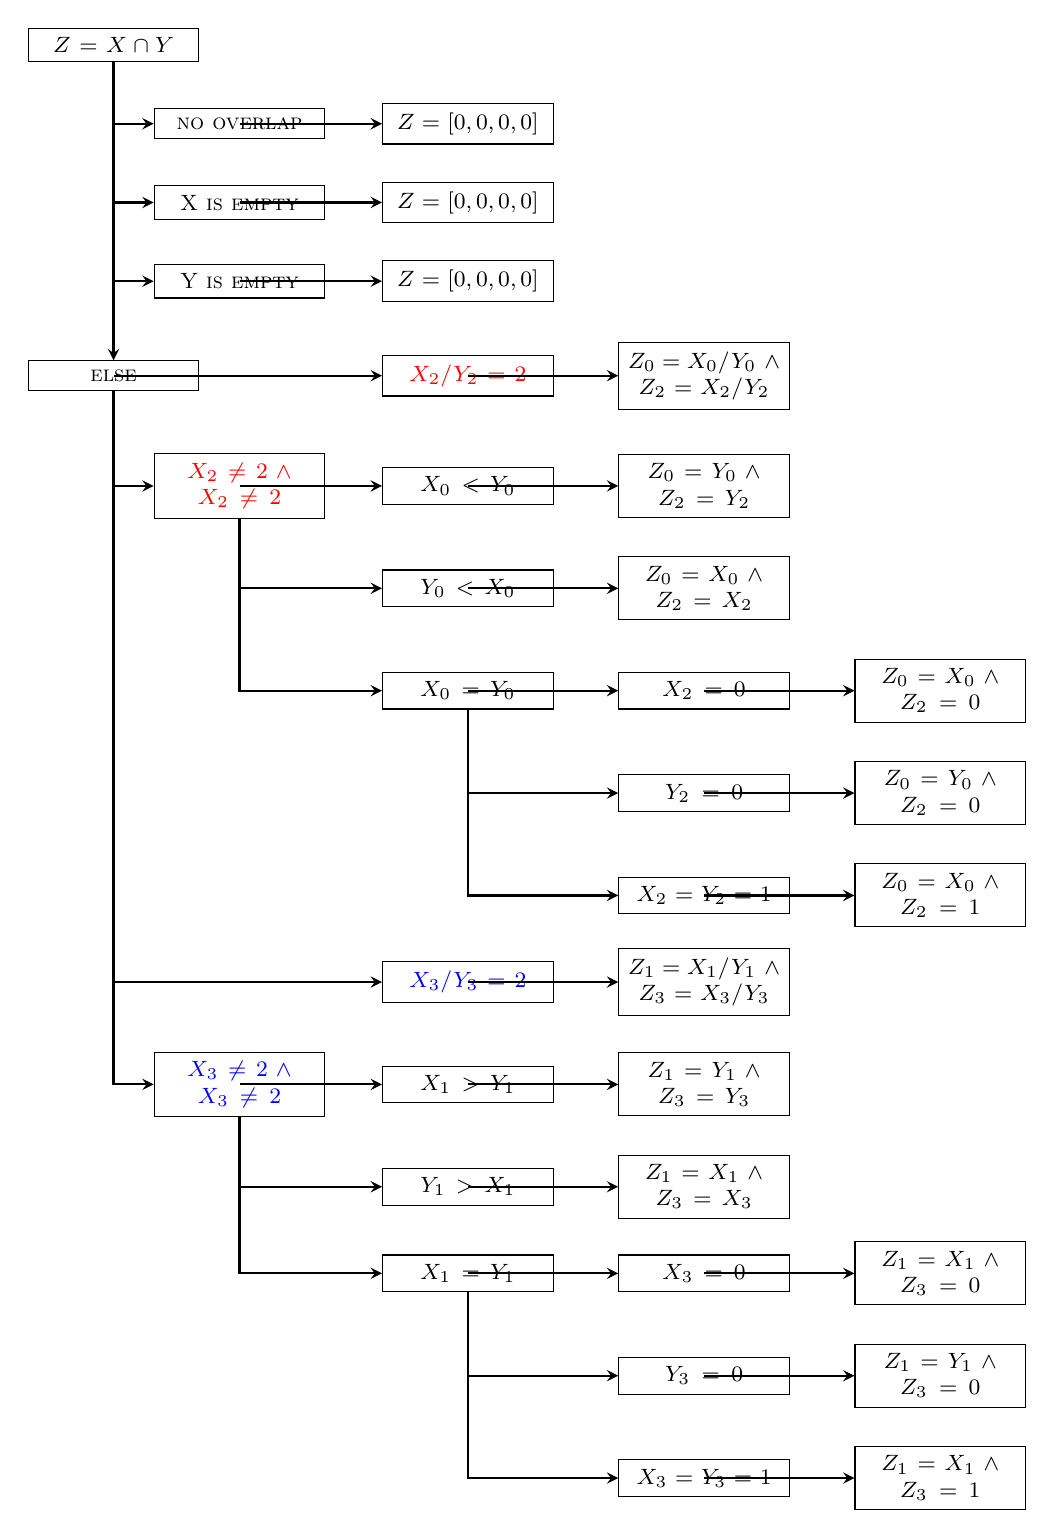
\begin{tikzpicture}[auto, >=latex, font=\footnotesize\scshape]
		\tikzstyle{center} = [draw=black, rectangle, text width=5.5em, align=center]
		\tikzstyle{centert} = [draw=black, rectangle, text width=5.5em, align=center, text=red]
		\tikzstyle{centerb} = [draw=black, rectangle, text width=5.5em, align=center, text=blue]
		\tikzstyle{arrow} = [thick,->,>=stealth]
		
		\node[center]	at (0, 8) 		(q0) 	{$Z = X \cap Y$};
		\node[center]	at (0, 3.8)		(q4)	{else};
		
		\node[center]	at (1.6, 7)		(q1)	{no overlap};
		\node[center]	at (1.6, 6) 	(q2) 	{X is empty};
		\node[center]	at (1.6, 5)		(q3)	{Y is empty};
		
		\node[centert]	at (1.6, 2.4)	(q6)	{$X_2 \ne 2$ $\land$ \\ $X_2 \ne 2$};
		\node[centerb]	at (1.6, -5.2)	(q7)	{$X_3 \ne 2$ $\land$ \\ $X_3 \ne 2$};
		
		\node[center]	at (4.5, 7)		(q9)	{$Z = [0, 0, 0, 0]$};
		\node[center]	at (4.5, 6)		(q10)	{$Z = [0, 0, 0, 0]$};
		\node[center]	at (4.5, 5)		(q11)	{$Z = [0, 0, 0, 0]$};
		\node[centert]	at (4.5, 3.8)	(q12)	{$X_2/Y_2 = 2$};
		\node[center]	at (4.5, 2.4)	(q14)	{$X_0 < Y_0$};
		\node[center]	at (4.5, 1.1)	(q15)	{$Y_0 < X_0$};
		\node[center]	at (4.5, -0.2)	(q16)	{$X_0 = Y_0$};
		\node[centerb]	at (4.5, -3.9)	(q13)	{$X_3/Y_3 = 2$};
		\node[center]	at (4.5, -5.2)	(q17)	{$X_1 > Y_1$};
		\node[center]	at (4.5, -6.5)	(q18)	{$Y_1 > X_1$};
		\node[center]	at (4.5, -7.6)	(q19)	{$X_1 = Y_1$};
		
		\node[center]	at (7.5, 3.8)		(q32)	{$Z_0 = X_0/Y_0$ $\land$ \\ $Z_2 = X_2/Y_2$};
		\node[center]	at (7.5, 2.4)		(q22)	{$Z_0 = Y_0$ $\land$ \\ $Z_2 = Y_2$};
		\node[center]	at (7.5, 1.1)		(q23)	{$Z_0 = X_0$ $\land$ \\ $Z_2 = X_2$};
		\node[center]	at (7.5, -0.2)		(q24)	{$X_2 = 0$};
		\node[center]	at (7.5, -1.5)		(q25)	{$Y_2 = 0$};
		\node[center]	at (7.5, -2.8)		(q26)	{$X_2 = Y_2 = 1$};
		\node[center]	at (7.5, -3.9)		(q33)	{$Z_1 = X_1/Y_1$ $\land$ \\ $Z_3 = X_3/Y_3$};
		\node[center]	at (7.5, -5.2)		(q27)	{$Z_1 = Y_1$ $\land$ \\ $Z_3 = Y_3$};
		\node[center]	at (7.5, -6.5)		(q28)	{$Z_1 = X_1$ $\land$ \\ $Z_3 = X_3$};
		\node[center]	at (7.5, -7.6)		(q29)	{$X_3 = 0$};
		\node[center]	at (7.5, -8.9)		(q30)	{$Y_3 = 0$};
		\node[center]	at (7.5, -10.2)		(q31)	{$X_3 = Y_3 = 1$};
		
		\node[center]	at (10.5, -0.2)	 (q35)	{$Z_0 = X_0$ $\land$ \\ $Z_2 = 0$};
		\node[center]	at (10.5, -1.5)	 (q36)	{$Z_0 = Y_0$ $\land$ \\ $Z_2 = 0$};
		\node[center]	at (10.5, -2.8)	 (q37)	{$Z_0 = X_0$ $\land$ \\ $Z_2 = 1$};
		\node[center]	at (10.5, -7.6)	 (q38)	{$Z_1 = X_1$ $\land$ \\ $Z_3 = 0$};
		\node[center]	at (10.5, -8.9)	 (q39)	{$Z_1 = Y_1$ $\land$ \\ $Z_3 = 0$};
		\node[center]	at (10.5, -10.2) (q40)	{$Z_1 = X_1$ $\land$ \\ $Z_3 = 1$};
		
		\draw [arrow] (q0)  -- (q4);
		
		\draw [arrow] (q0)  |- (q1);
		\draw [arrow] (q0)  |- (q2);
		\draw [arrow] (q0)  |- (q3);
		
		\draw [arrow] (q4)  |- (q6);
		\draw [arrow] (q4)  |- (q7);
		
		\draw [arrow] (q1)  |- (q9);
		\draw [arrow] (q2)  |- (q10);
		\draw [arrow] (q3)  |- (q11);
		\draw [arrow] (q4)  |- (q12);
		\draw [arrow] (q4)  |- (q13);
		\draw [arrow] (q6)  |- (q14);
		\draw [arrow] (q6)  |- (q15);
		\draw [arrow] (q6)  |- (q16);
		\draw [arrow] (q7)  |- (q17);
		\draw [arrow] (q7)  |- (q18);
		\draw [arrow] (q7)  |- (q19);
		
		\draw [arrow] (q12) |- (q32);
		\draw [arrow] (q13) |- (q33);
		\draw [arrow] (q14) |- (q22);
		\draw [arrow] (q15) |- (q23);
		\draw [arrow] (q16) |- (q24);
		\draw [arrow] (q16) |- (q25);
		\draw [arrow] (q16) |- (q26);
		\draw [arrow] (q17) |- (q27);
		\draw [arrow] (q18) |- (q28);
		\draw [arrow] (q19) |- (q29);
		\draw [arrow] (q19) |- (q30);
		\draw [arrow] (q19) |- (q31);
		
		\draw [arrow] (q24) |- (q35);
		\draw [arrow] (q25) |- (q36);
		\draw [arrow] (q26) |- (q37);
		\draw [arrow] (q29) |- (q38);
		\draw [arrow] (q30) |- (q39);
		\draw [arrow] (q31) |- (q40);
		
	\end{tikzpicture}
	\caption{Overview of the interval intersection operation}
	\label{fig:intersection}
\end{figure}

If neither X or Y goes to infinity we will look at whether or not either bound is further out than the other. If this is the case than the most inner side will be chosen to be the representative for that bound in Z. 

If both bounds are equal then we look if they are both inclusive, if yes then Z will be inclusive too, if either one is not inclusive then Z will also be not inclusive for said bound. The value of Z will be equal to the bound of X and Y in any of these cases.

\subsubsection{Interval union}
The union operation is summarised in Figure \ref{fig:union} below. We can immediately see that this is very similar to the intersection in the sense that most of the conditional statements are the exact same. 

\begin{figure}
	\centering
	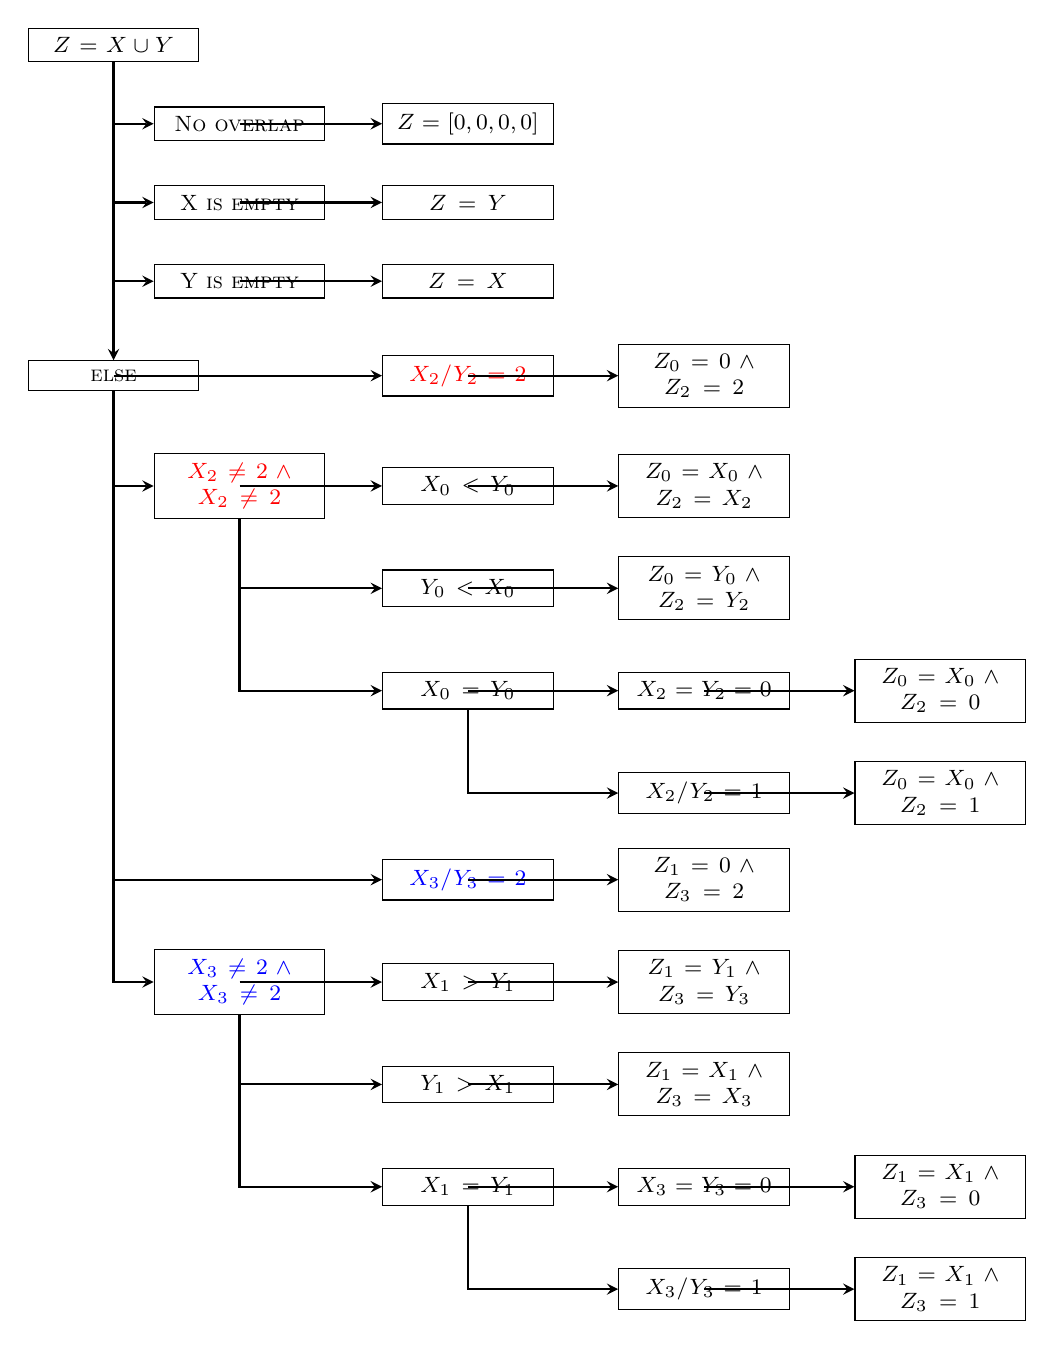
\begin{tikzpicture}[auto, >=latex, font=\footnotesize\scshape]
		\tikzstyle{center} = [draw=black, rectangle, text width=5.5em, align=center]
		\tikzstyle{centert} = [draw=black, rectangle, text width=5.5em, align=center, text=red]
		\tikzstyle{centerb} = [draw=black, rectangle, text width=5.5em, align=center, text=blue]
		\tikzstyle{arrow} = [thick,->,>=stealth]
		
		\node[center]	at (0, 8) 		(q0) 	{$Z = X \cup Y$};
		\node[center]	at (0, 3.8)		(q4)	{else};
		
		\node[center] 	at (1.6, 7)		(q5)	{No overlap};		
		\node[center]	at (1.6, 6) 	(q2) 	{X is empty};
		\node[center]	at (1.6, 5)		(q3)	{Y is empty};
		
		\node[centert]	at (1.6, 2.4)	(q6)	{$X_2 \ne 2$ $\land$ \\ $X_2 \ne 2$};
		\node[centerb]	at (1.6, -3.9)	(q7)	{$X_3 \ne 2$ $\land$ \\ $X_3 \ne 2$};
		
		\node[center]	at (4.5, 7)		(q9)	{$Z = [0, 0, 0, 0]$};
		\node[center]	at (4.5, 6)		(q10)	{$Z = Y$};
		\node[center]	at (4.5, 5)		(q11)	{$Z = X$};
		\node[centert]	at (4.5, 3.8)	(q12)	{$X_2/Y_2 = 2$};
		\node[center]	at (4.5, 2.4)	(q14)	{$X_0 < Y_0$};
		\node[center]	at (4.5, 1.1)	(q15)	{$Y_0 < X_0$};
		\node[center]	at (4.5, -0.2)	(q16)	{$X_0 = Y_0$};
		\node[centerb]	at (4.5, -2.6)	(q13)	{$X_3/Y_3 = 2$};
		\node[center]	at (4.5, -3.9)	(q17)	{$X_1 > Y_1$};
		\node[center]	at (4.5, -5.2)	(q18)	{$Y_1 > X_1$};
		\node[center]	at (4.5, -6.5)	(q19)	{$X_1 = Y_1$};
		
		\node[center]	at (7.5, 3.8)		(q32)	{$Z_0 = 0$ $\land$ \\ $Z_2 = 2$};
		\node[center]	at (7.5, 2.4)		(q22)	{$Z_0 = X_0$ $\land$ \\ $Z_2 = X_2$};
		\node[center]	at (7.5, 1.1)		(q23)	{$Z_0 = Y_0$ $\land$ \\ $Z_2 = Y_2$};
		\node[center]	at (7.5, -0.2)		(q25)	{$X_2 = Y_2 = 0$};
		\node[center]	at (7.5, -1.5)		(q26)	{$X_2/Y_2 = 1$};
		\node[center]	at (7.5, -2.6)		(q33)	{$Z_1 = 0$ $\land$ \\ $Z_3 = 2$};
		\node[center]	at (7.5, -3.9)		(q27)	{$Z_1 = Y_1$ $\land$ \\ $Z_3 = Y_3$};
		\node[center]	at (7.5, -5.2)		(q28)	{$Z_1 = X_1$ $\land$ \\ $Z_3 = X_3$};
		\node[center]	at (7.5, -6.5)		(q30)	{$X_3 = Y_3 = 0$};
		\node[center]	at (7.5, -7.8)		(q31)	{$X_3/Y_3 = 1$};
		
		\node[center]	at (10.5, -0.2)	 (q36)	{$Z_0 = X_0$ $\land$ \\ $Z_2 = 0$};
		\node[center]	at (10.5, -1.5)	 (q37)	{$Z_0 = X_0$ $\land$ \\ $Z_2 = 1$};
		\node[center]	at (10.5, -6.5)	 (q39)	{$Z_1 = X_1$ $\land$ \\ $Z_3 = 0$};
		\node[center]	at (10.5, -7.8) (q40)	{$Z_1 = X_1$ $\land$ \\ $Z_3 = 1$};
		
		\draw [arrow] (q0)  -- (q4);
		
		\draw [arrow] (q0)	|- (q5);
		\draw [arrow] (q0)  |- (q2);
		\draw [arrow] (q0)  |- (q3);		
		\draw [arrow] (q4)  |- (q6);
		\draw [arrow] (q4)  |- (q7);
		
		\draw [arrow] (q5)  |- (q9);
		\draw [arrow] (q2)  |- (q10);
		\draw [arrow] (q3)  |- (q11);
		\draw [arrow] (q4)  |- (q12);
		\draw [arrow] (q4)  |- (q13);
		\draw [arrow] (q6)  |- (q14);
		\draw [arrow] (q6)  |- (q15);
		\draw [arrow] (q6)  |- (q16);
		\draw [arrow] (q7)  |- (q17);
		\draw [arrow] (q7)  |- (q18);
		\draw [arrow] (q7)  |- (q19);
		
		\draw [arrow] (q12) |- (q32);
		\draw [arrow] (q13) |- (q33);
		\draw [arrow] (q14) |- (q22);
		\draw [arrow] (q15) |- (q23);
		\draw [arrow] (q16) |- (q25);
		\draw [arrow] (q16) |- (q26);
		\draw [arrow] (q17) |- (q27);
		\draw [arrow] (q18) |- (q28);
		\draw [arrow] (q19) |- (q30);
		\draw [arrow] (q19) |- (q31);
		
		\draw [arrow] (q25) |- (q36);
		\draw [arrow] (q26) |- (q37);
		\draw [arrow] (q30) |- (q39);
		\draw [arrow] (q31) |- (q40);
		
	\end{tikzpicture}
	\caption{Overview of the interval union operation}
	\label{fig:union}
\end{figure}


We once again split the evaluation into two near identical evaluations being marked by the blue and red nodes. The red segment relates to the lower bound, the blue segment to the upper bound. In case either side goes to infinity for $X$ or $Y$, $Z$ will trivially go to infinity too. In case it does not go to infinity we will select the one closest to the bounds. Finally if both bounds are equal we will by default set the boundary value equal to the boundary value of $X$ and $Y$ and make it inclusive if either $X$ or $Y$ are inclusive and exclusive otherwise.

\subsubsection{Interval progression}
For further intervals to get populated we need conditions to represent the potential traversal of edges. Note that we do not consider an actual path through the automaton, we simply try to guess a configuration. We do not require our solver to give us a unique or optimal solution, we simply require the resulting configuration to represent a subset of all reachable counter values for which the node under test is proven to be reachable.

Each sub interval can either be empty, in case there are no transitions that can be activated, or it holds the result of an update. The schema given in Figure \ref{fig:int progression 1} describes the logic which is applied on the sub intervals. Given that we are currently evaluating sub interval $i$ of node $q$ we can see that it will be empty in case no transitions can fire. If a transition can still fire the interval will be equal to the direct result of an update starting from the sub interval $j$ of a node $p$ given that there is a transition $t$ going from $p$ to $q$. 

\begin{figure}[h]
	\centering
	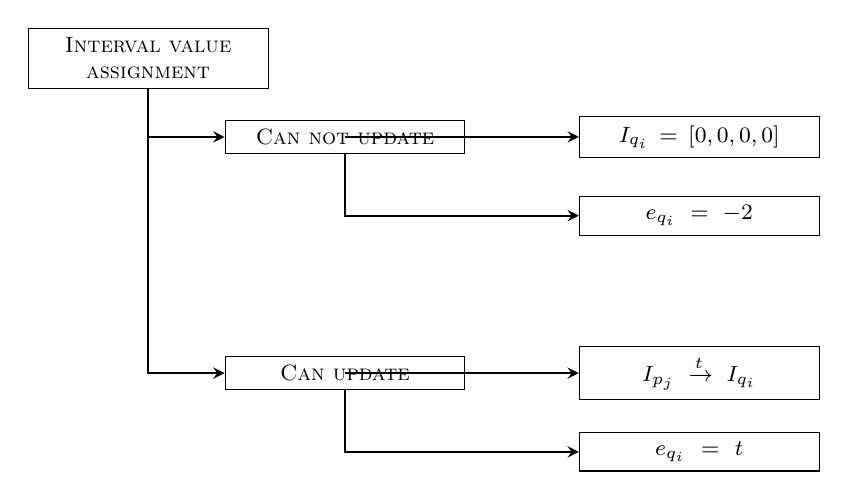
\begin{tikzpicture}[auto, >=latex, font=\footnotesize\scshape]
		\tikzstyle{small} = [draw=black, rectangle]
		\tikzstyle{center} = [draw=black, rectangle, text width=8em, align=center]
		\tikzstyle{arrow} = [thick,->,>=stealth]
		
		\node[center]	at (0, 0) 		(q0) 	{Interval value assignment};
		
		\node[center]	at (2.5, -1) 	(q3)	{Can not update};
		\node[center]	at (2.5, -4)	(q4)	{Can update};
		
		\node[center]	at (7, -2)		(q5)	{$e_{q_i} = -2$};
		\node[center]	at (7, -1)		(q6) 	{$I_{q_i}  = [0, 0, 0, 0]$};
		\node[center]	at (7, -5)		(q7)	{$e_{q_i} = t$};
		\node[center] 	at (7, -4)		(q9)	{$I_{p_j} \xrightarrow{t} I_{q_i}$};
		
		\draw [arrow] (q0) |- (q3);
		\draw [arrow] (q0) |- (q4);
		
		\draw [arrow] (q3) |- (q5);
		\draw [arrow] (q3) |- (q6);
		
		\draw [arrow] (q4) |- (q7);
		\draw [arrow] (q4) |- (q9);
	\end{tikzpicture}
	\caption{Overview of the interval assignment conditions}
	\label{fig:int progression 1}
\end{figure}

We will furthermore ensure that a transition $t$ can only be used once per node $q$. This is done as to prevent needlessly filling each subinterval. 

The \textit{can update} condition will be applied on a preceding interval $I_{p_j}$ and a current interval $I_{q_i}$. First of all we will check that neither $I_{p_j}$ and $I_{q_i}$ are empty. If either of the two are empty we do not consider it as an update and the update will not be marked as possible.

\begin{gather*}
	\hspace{-6 pt} succ_{p, q}(R_i) := \bigcup \{(R_i(p, q) + (0, z]) \cap \tau(q)\,|\,(p,z,q) \in T, z>0\}\\
	\hspace{60 pt} \cup \bigcup \{(R_i(p, q) + (z, 0]) \cap \tau(q)\,|\,(p,z,q) \in T, z<0\}\\
	\hspace{-20 pt} \cup \bigcup \{R_i(p, q) \cap \tau(q)\,|\,(p,0,q) \in T\}
\end{gather*}

Next we will follow the same \textit{succ} function as we followed for the reachability of non-parametric COCA. For this function to be applied we will make use of two additional helper intervals called Y and Y2, which will need to be instantiated for each evaluated edge. The first step will be the addition which is dependent on the the $z$ variable representing the edge operation. In Figure \ref{fig:int progression 2} below this interval is simply denoted as \textit{addend}.

\begin{figure}[b!]
	\centering
	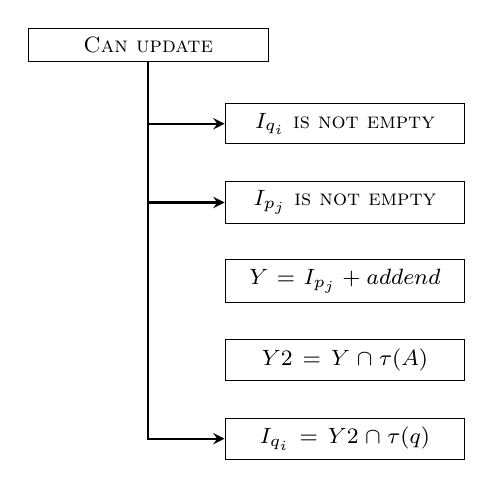
\begin{tikzpicture}[auto, >=latex, font=\footnotesize\scshape]
		\tikzstyle{small} = [draw=black, rectangle]
		\tikzstyle{center} = [draw=black, rectangle, text width=8em, align=center]
		\tikzstyle{arrow} = [thick,->,>=stealth]
		
		\node[center]	at (0, 0) 		(q0) 	{Can update};
		
		\node[center]	at (2.5, -1) 	(q3)	{$I_{q_i}$ is not empty};
		\node[center]	at (2.5, -2)	(q4)	{$I_{p_j}$ is not empty};
		\node[center] 	at (2.5, -3)	(q5)	{$Y = I_{p_j} + addend$};
		\node[center] 	at (2.5, -4)	(q5)	{$Y2 = Y \cap \tau(A)$};
		\node[center] 	at (2.5, -5)	(q5)	{$I_{q_i} = Y2 \cap \tau(q)$};
		
		\draw [arrow] (q0) |- (q3);
		\draw [arrow] (q0) |- (q4);
		\draw [arrow] (q0) |- (q5);
	\end{tikzpicture}
	\caption{Overview of the can update condition}
	\label{fig:int progression 2}
\end{figure}

Next we will need to ensure that Y does not exceed any of the bounds. This will be done by first of all intersecting Y with the bounds of the automaton A. The result of this will be stored in Y2 which will then once again be intersected but this time with the bounds of the node q in which the edge ends. The result of this final intersection will be stored in $I_{q_i}$.

We have thus evaluated whether or not an update is possible. If so, the interval $I_{q_i}$ will trivially hold the result of this update, if not the initial interval assignment condition visualised in Figure \ref{fig:int progression 1} will let the interval be equal to the empty interval. We can therefore remove the condition saying that $I_{q_i}$ must hold the result of taking the transition $t$ from interval $I_{p_j}$.

Finally, in case one wishes to compute the reachability interval of an entire node we can simply consider the union of all subintervals.

\begin{figure}[h]%
	\centering
	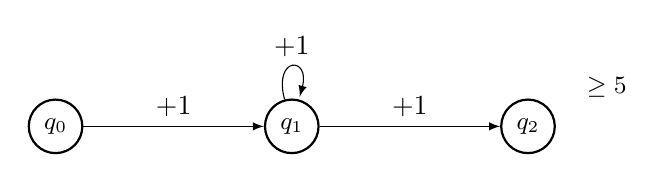
\begin{tikzpicture}[auto, >=latex, node distance = 1 cm]
		\tikzstyle{round} = [thick, draw=black, circle, font=\small]
		\tikzstyle{invis} = [draw=none, font=\small]
		\tikzstyle{arrow} = [thick,->,>=stealth]
		
		\node[round] 	at (0, 0) 		(q0) 	{$q_0$};
		\node[round] 	at (3, 0)		(q1) 	{$q_1$};
		\node[round] 	at (6, 0)		(q2) 	{$q_2$};
		\node[invis]	at (7, 0.5)		(q4)	{$\geq 5$};
		
		\path[->]
		(q0) 	edge 					node 					{$+1$}	(q1)
		(q1) 	edge 					node 					{$+1$}	(q2)
		(q1)	edge 	[loop above]	node					{$+1$}	(q1);
	\end{tikzpicture}
	\caption{Example of an automaton with a loop}
	\label{fig:example loop}
\end{figure}

If we consider the automaton given in Figure \ref{fig:example loop} we start with only $q_0$ being reachable with one of its subintervals equal to the interval $[0, 0]$ or the configuration $0, 0, 1, 1$ in formula format. 

There will be conditions for each of the subintervals $I_{q_{1_{i}}}$ of node $q_1$ stating that if there exists an interval $I_{q_{0_{j}}}$ of node $q_0$ on which the edge operation $+1$ can be applied, we should do so. Given our current context this is indeed possible and we will therefore assign $0, 1, 0, 1$ to one of the subintervals of $q_1$ as this will be the resulting value. The corresponding edge value will be set equal to 0, given that the first edge is labelled $0$.

The same condition will exist for $q_1$ but now requiring there to both be a resulting interval and preceding interval part of $q_1$. Given that this loop only has an addition and no subtractions, any interval going to positive infinity could be used as a fix point for it. In this case $0, 0, 0, 2$ or $(0, \infty)$ was chosen to represent both the preceding and resulting interval.

\begin{table*}[b]
	\centering
	\begin{tabular}{ |c|c|c|c|  }
		\hline
		& q0 				& q1 			& q2 \\
		\hline
		Interval 1 	& -1: 0, 0, 1, 1	& 0: 0, 1, 0, 1 & 2: 5, 0, 1, 2 \\
		\hline
		Interval 2 	& -2: 0, 0, 0, 0	& 1: 0, 0, 0, 2 & -2: 0, 0, 0, 0 \\
		\hline
	\end{tabular}
	\caption{Example interval configuration post evaluation}
	\label{table:example loop intervals}
\end{table*}

Finally, the edge between $q_1$ and $q_2$, labelled edge 2, can be taken if there is a sub interval $I_{q_{1_i}}$ part of $q_1$ and a sub interval $I_{q_{2_j}}$ part of $q_2$ for which the conditions hold. If we consider the interval generated from edge 1 we can apply edge 2 to this and get the resulting interval $0, 0, 0, 2$. This does however not satisfy the node bound that exist on $q_2$ and thus our resulting interval will be $5, 0, 1, 2$ which does satisfy.

After assigning all of these intervals we get the results in Table \ref{table:example loop intervals} where all intervals are given using the format $<edge>: <interval>$. Note that there are many more intervals that are simply left out as they are all empty.

\subsubsection{Loop progression}
In case we only use the conditions above we will still have a problem with loops. Considering the example below in Figure \ref{fig:example loop bounded}, node $q_2$ is not reachable as our initial value is equal to 0 and we only have positive operations. However, with the condition given above any interval with an upper bound equal to $\infty$ would work as a fix point. We can therefore perfectly select the interval $(-20, \infty)$ and the conditions would be satisfied. We should therefore add an additional condition that restricts fix points for loops.

\begin{figure}[h]%
	\centering
	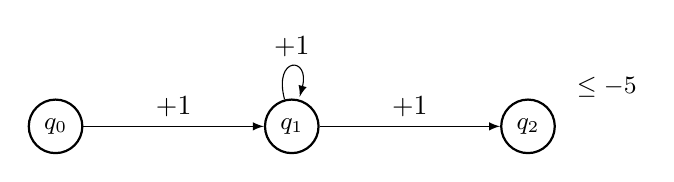
\begin{tikzpicture}[auto, >=latex, node distance = 1 cm]
		\tikzstyle{round} = [thick, draw=black, circle, font=\small]
		\tikzstyle{invis} = [draw=none, font=\small]
		\tikzstyle{arrow} = [thick,->,>=stealth]
		
		\node[round] 	at (0, 0) 		(q0) 	{$q_0$};
		\node[round] 	at (3, 0)		(q1) 	{$q_1$};
		\node[round] 	at (6, 0)		(q2) 	{$q_2$};
		\node[invis]	at (7, 0.5)		(q4)	{$\leq -5$};
		
		\path[->]
		(q0) 	edge 					node 					{$+1$}	(q1)
		(q1) 	edge 					node 					{$+1$}	(q2)
		(q1)	edge 	[loop above]	node					{$+1$}	(q1);
	\end{tikzpicture}
	\caption{Example of an automaton with a loop that needs to be restricted}
	\label{fig:example loop bounded}
\end{figure}

Considering the definitions of loop expansion given in Section \textit{\ref{sec:accel} \nameref{sec:accel}} we will differentiate between the different types of expanding loops. Consider a loop $l$ with transitions $t_0, t_1, ..., t_k$ which goes over the nodes $q_i, q_i+1, ..., q_j$. We furthermore assume that the interval with index 0 of each of the nodes will be used to represent the loop. Finally, we assume to be working in an automaton which has $n$ intervals per node. An overview of the conditions that need to be enforced in case loops are present can be seen in Figure \ref{fig:loop condition}.

In case the loop under consideration is not taken the condition should trivially evaluate to true. In case it is taken there should be at least one node that has an interval that is not related to the loop (the intervals related to the loop are at index 0 and are therefore not considered in the equation). If it is not expanding in either direction it has to originate in another existing interval and it should therefore be bounded by the values part of any other interval. The $min\_val$ and $max\_val$ variables are computed using the formulae below.

\begin{gather*}
	\text{min\_val}_q = min(I_{{q_1}_{low}}, I_{{q_2}_{low}}, ..., I_{{q_n}_{low}})\\
	\text{max\_val}_q = max(I_{{q_1}_{high}}, I_{{q_2}_{high}}, ..., I_{{q_n}_{high}})
\end{gather*}

In case either the min or max variable go to infinity, the conditions for their respective bounds should trivially be satisfied as the intervals are no longer bounded in that case. The schema representing the loop condition can be found below in Figure \ref{fig:loop condition}.

\begin{figure}[h]
	\centering
	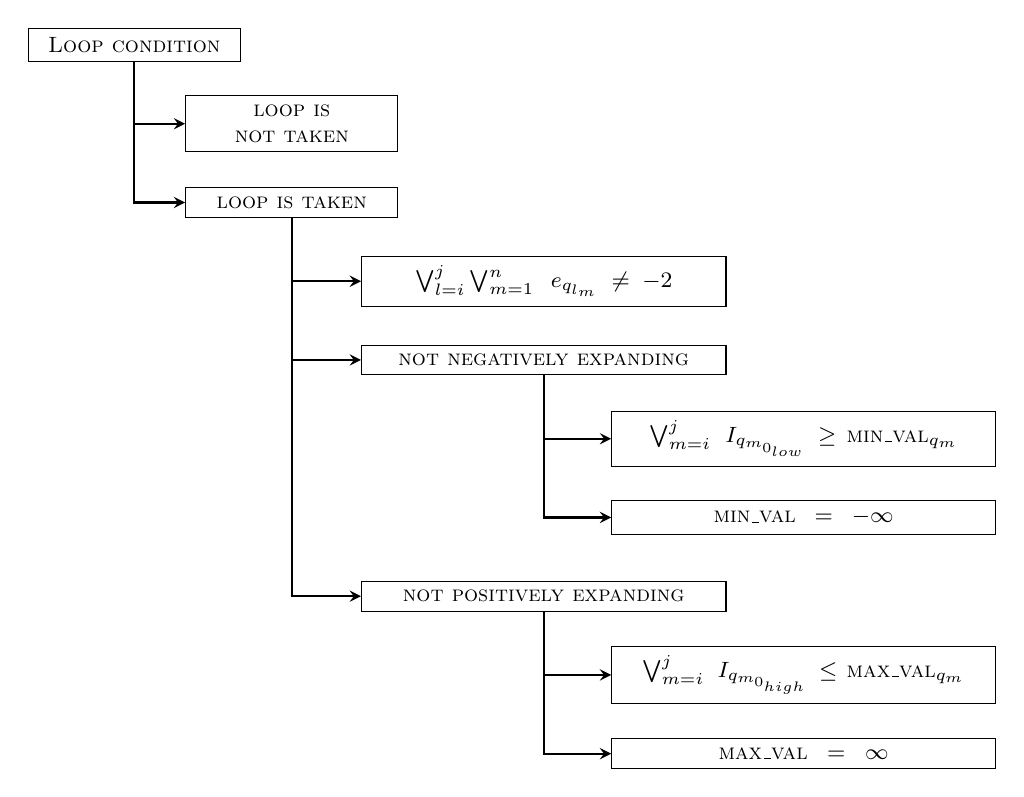
\begin{tikzpicture}[auto, >=latex, font=\footnotesize\scshape]
		\tikzstyle{small} = [draw=black, rectangle]
		\tikzstyle{centersmall} = [draw=black, rectangle, text width=7em, align=center]
		\tikzstyle{center} = [draw=black, rectangle, text width=12.5em, align=center]
		\tikzstyle{centerlarge} = [draw=black, rectangle, text width=13.2em, align=center]
		\tikzstyle{arrow} = [thick,->,>=stealth]
		
		\node[centersmall]	at (0, 0) 		(q0) 	{Loop condition};
		
		\node[centersmall]	at (2, -1) 		(q3)	{loop is not taken};
		\node[centersmall]	at (2, -2)		(q4)	{loop is taken};
		
		\node[center]		at (5.2, -3)	(q5)	{$\bigvee_{l = i}^{j}\bigvee_{m = 1}^{n}\;e_{q_{l_m}} \ne -2$};
		\node[center]		at (5.2, -4)	(q6)	{not negatively expanding};
		\node[center]		at (5.2, -7)	(q7)	{not positively expanding};
		
		\node[centerlarge]		at (8.5, -5)	(q8)	{$\bigvee_{m = i}^{j}\;I_{q_{m_{0_{low}}}} \geq \text{min\_val}_{q_m}$};
		\node[centerlarge]		at (8.5, -6)	(q9)	{$\text{min\_val} = -\infty$};
		\node[centerlarge]		at (8.5, -8)	(q10)	{$\bigvee_{m = i}^{j}\;I_{q_{m_{0_{high}}}} \leq \text{max\_val}_{q_m}$};
		\node[centerlarge]		at (8.5, -9)	(q11)	{$\text{max\_val} = \infty$};
		
		\draw [arrow] (q0) |- (q3);
		\draw [arrow] (q0) |- (q4);
		
		\draw [arrow] (q4) |- (q5);
		\draw [arrow] (q4) |- (q6);
		\draw [arrow] (q4) |- (q7);
		
		\draw [arrow] (q6) |- (q8);
		\draw [arrow] (q6) |- (q9);
		\draw [arrow] (q7) |- (q10);
		\draw [arrow] (q7) |- (q11);
	\end{tikzpicture}
	\caption{Overview of the loop condition}
	\label{fig:loop condition}
\end{figure}

When we now reinvestigate the example in Figure \ref{fig:example loop bounded} we can get the intervals given in Table \ref{table:example loop bounded intervals}. Note our edges are numerically labelled here. The label 0 represents the edge from $q_0$ to $q_1$, label 1 represents the loop and label 2 represents the edge from $q_1$ to $q_2$. Instead of going negative the node $q_1$ will now go from 0 to infinity and node $q_2$ will thus not be discovered as being reachable which is as expected. The second interval of $q_1$ can never go negative as it would then fail to satisfy the loop conditions given above.

\begin{table*}[t]
	\centering
	\begin{tabular}{ |c|c|c|c|  }
		\hline
		& q0 				& q1 			& q2 \\
		\hline
		Interval 1 	& -1: 0, 0, 1, 1	& 0: 0, 1, 0, 1 & -2: 0, 0, 0, 0 \\
		\hline
		Interval 2 	& -2: 0, 0, 0, 0	& 1: 0, 0, 0, 2 & -2: 0, 0, 0, 0 \\
		\hline
	\end{tabular}
	\caption{Example interval configuration post evaluation}
	\label{table:example loop bounded intervals}
\end{table*}

\section{Use case: xrdp}
Xrdp\footnote{\url{https://github.com/neutrinolabs/xrdp}} is a medium sized c project that provides a graphical login to remote machines using Microsoft Remote Desktop. It was chosen as a use case for this project as it is a real life example of a project that would greatly benefit from dead code elimination. It consists of 120 files containing 94 458 lines of code and there are a total of 1 328 functions (not including defines). It is interesting for dead code analysis as it is highly dependant on efficiency. It is furthermore used in several other projects as this project is forked into 947 repositories thus indicating that this project counts as a core reused in other projects. Inefficiencies in this project would be further extrapolated in the projects who inherit from it and should therefore be prevented at all costs.

\begin{table}[h]
	\centering
	\begin{tabular}{ |p{4.5cm}|r|  }
		\hline
		lines of code & 94 458\\
		\hline
		number of functions   & 1 328\\
		\hline
		number of forks   & 947\\
		\hline
	\end{tabular}
	\caption{Statistics for the xrdp project}
\end{table}


\subsection{shortcomings}
The code analysis quickly showed flaws in the compiler resulting from the first phase in the analysis.

A first major case that was found rather quickly were cases in which a function is used in conditional statements, rather than variables. This situation was not fully taken into account and will lead to false results. For example, there is an instance where a function is simply used as boolean within if statements. In these statements the validator should have returned that this case is not analysable, as we can not investigate whether or not the invoked function can return a certain value but instead the code will simply not acknowledge the function as a counter as it is programmed to only handle values. In the example in Listing \ref{lst:functional condition} we can see a case where a function is used on line 11 and 14 yet the one counter automaton will be generated but simply without any counter. For this analysis such results were manually removed to avoid analysing trivial cases with our new reachability approach.

\begin{lstlisting}[style=CStyle,caption={Example of code using functions as conditional values}, label={lst:functional condition}]
int
cleanup_sockets(int display)
{
	LOG(LOG_LEVEL_INFO, "cleanup_sockets:");
	char file[256];
	int error;
	
	error = 0;
	
	g_snprintf(file, 255, CHANSRV_PORT_OUT_STR, display);
	if (g_file_exist(file))
	{
		LOG(LOG_LEVEL_DEBUG, "cleanup_sockets: deleting %s", file);
		if (g_file_delete(file) == 0)
		{
			LOG(LOG_LEVEL_WARNING,
			"cleanup_sockets: failed to delete %s (%s)",
			file, g_get_strerror());
			error++;
		}
	}
}
\end{lstlisting}

Another issue that was found were data structures which the compiler did not recognize. Within the compiler structs are supported and optimizations using the different variables that are part of structs are performed. There is however no optimization for pointers to structs. 

When a variable points to a struct you will not access its members with the . operation but rather with the -$\textgreater$ operator. This is however not supported in the compiler and use of this operator will lead to exceptions where an optimization function attempts to optimize this without success. Another case were struct pointers have weird effects are cases such as in Listing \ref{lst:not considered condition}. In this case it will once again not detect any counter while in essence we are verifying whether or not the mod variable is initialized by the verification done on line 6.

\begin{lstlisting}[style=CStyle, caption={Example of comparisons not considered by the compiler}, label={lst:not considered condition}]
int
mod_exit(tintptr handle)
{
	struct mod *mod = (struct mod *) handle;
	
	if (mod == 0)
	{
		return 0;
	}
	
	g_free(mod);
	return 0;
}
\end{lstlisting}

Finally, an attempt was made to support dereferencing of pointers as well as pointers of pointers but immediate access during dereference was not considered during the writing of the compiler and will also lead to unhandled cases. In Listing \ref{lst:pointer access} the operation on line 4 where the \textit{fip} variable is dereferenced and directly accessed afterwards is not supported by the compiler. The function in Listing \ref{lst:pointer access} will lead to a direct crash of the compiler.

\begin{lstlisting}[style=CStyle, caption={Example of unsupported access to pointer values}, label={lst:pointer access}]
void xfuse_devredir_cb_enum_dir_done(struct state_dirscan *fip,
enum NTSTATUS IoStatus)
{
	struct fuse_file_info *fi = &fip->fi;
	XFUSE_HANDLE *xhandle = xfuse_handle_create();
	
	if (xhandle == NULL
	|| (xhandle->dir_handle = xfs_opendir(g_xfs, fip->pinum)) == NULL)
	{
		fuse_reply_err(fip->req, ENOMEM);
	}
}
\end{lstlisting}

Finally there were other cases where node mappings occurred that were not expected possible. For example, arguments that are not structs are mapped as is visualised in Image \ref{fig:normal arguments}. However, when this type is a struct an entirely different format is used as can be seen in Figure \ref{fig:struct arguments}.

\begin{figure}[h]
	\centering
	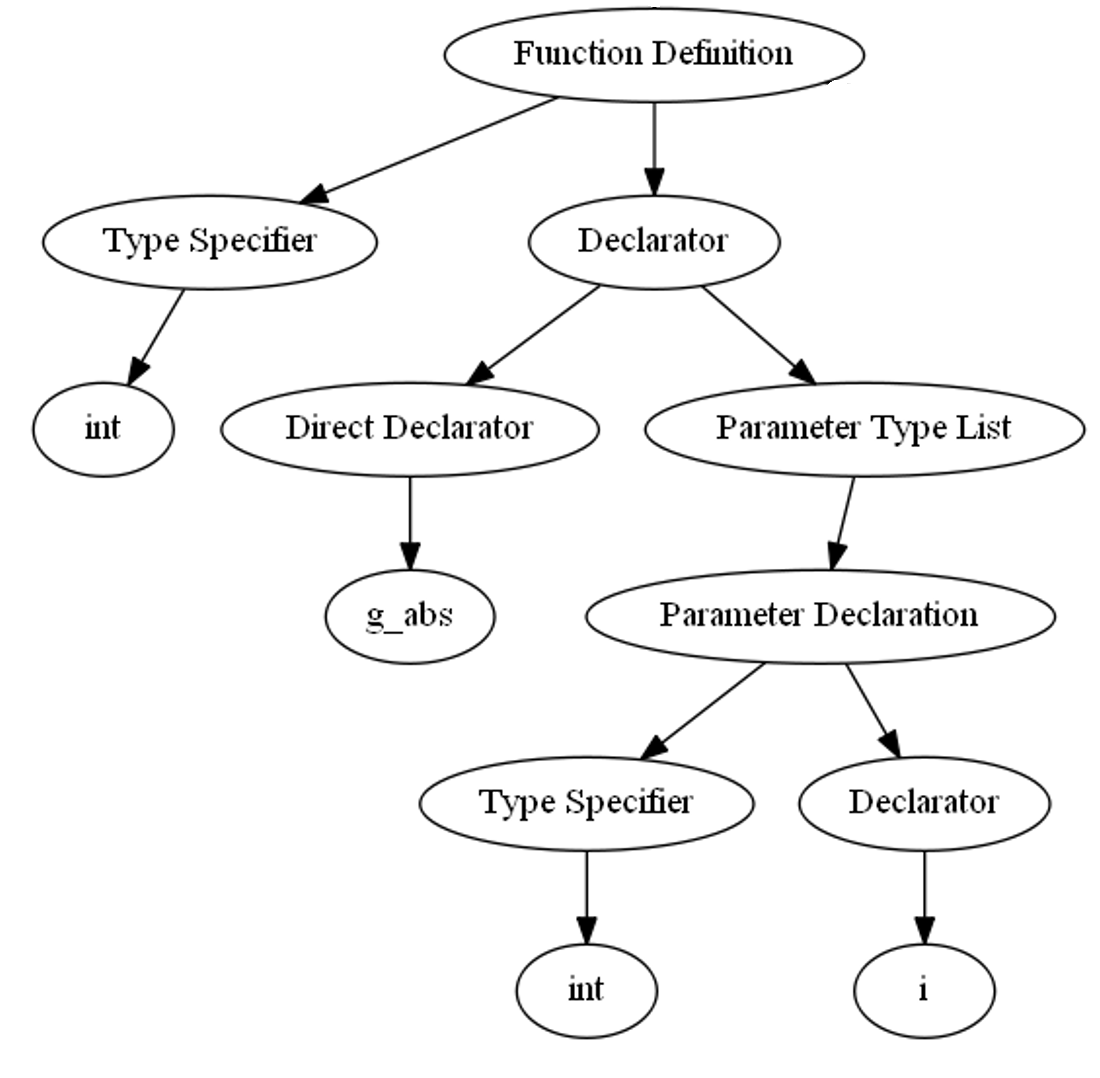
\includegraphics[width=0.4\linewidth]{images/normal_function_param.png}
	\caption{Function with normal argument format}
	\label{fig:normal arguments}
\end{figure}


\begin{figure}[h]
	\centering
	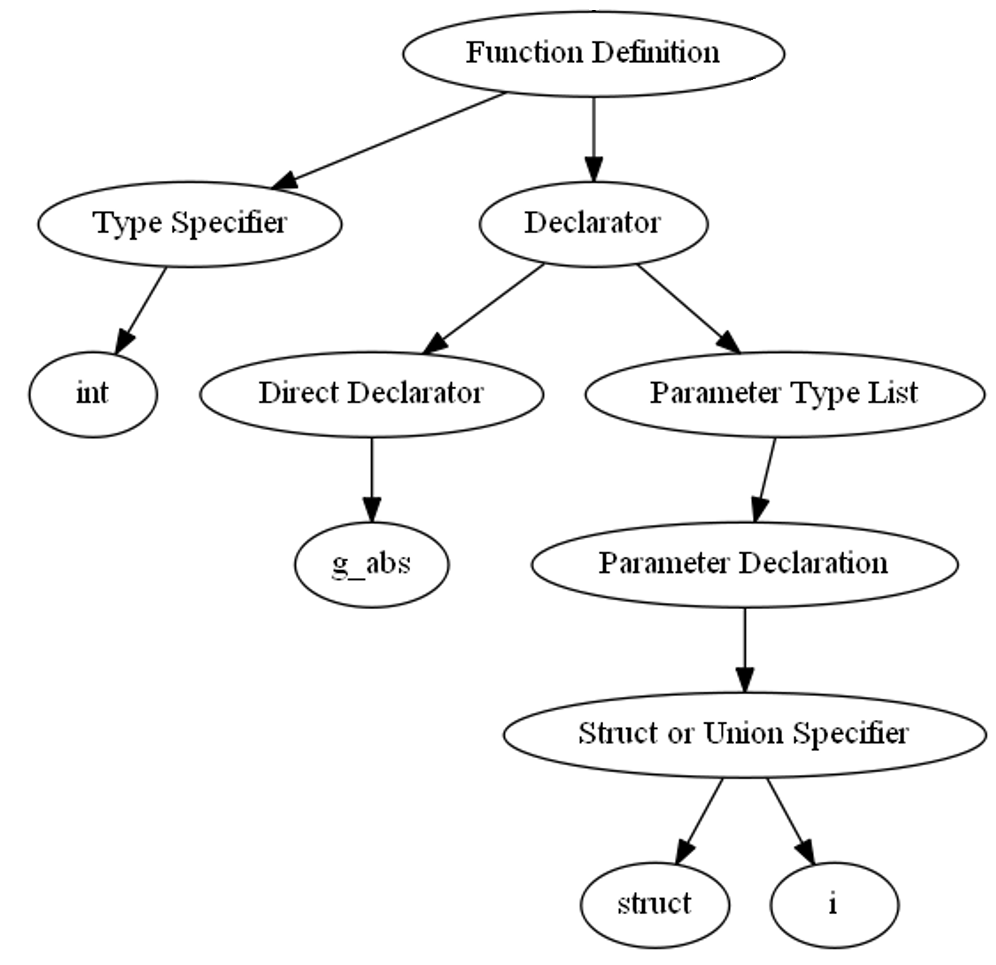
\includegraphics[width=0.4\linewidth]{images/not_normal_function_param.png}
	\caption{Function with struct argument format}
	\label{fig:struct arguments}
\end{figure}

In the initial compiler the first format was assumed and thus several errors occurred due to missing nodes during the evaluation of the project. This is very hard to consider beforehand and cases like this make it near impossible to properly identify every possible case that can ever occur. A significant amount of errors of this kind were resolved, such as this one, but not all.

\subsection{Results}
As a result of these issues several files were not analysable. An attempt was made to resolve as many issues as possible such as the lack of proper preprocessing. Some of the optimizations were also disabled, such as optimizations for variable types which can not be handled by the compiler but this eventually resulted in other components breaking. This leads to 76 files of the 120 total files being evaluated correctly. Within these files a total of 975 functions were evaluated of which 35 were found to be suitable for counter evaluation. Two of these functions had a function in their conditional statement and should not have been accepted for counter automaton analysis. All other cases were correctly identified and were all ready for further analysis.

\begin{table}[h]
	\centering
	\begin{tabular}{ |p{4.5cm}|c|c|c|  }
		\hline
		Metric 				& Actual & Found & Percentage\\
		\hline
		Number of files 	& 120	 & 76 & 63.33\%\\
		\hline
		Number of functions & 1 328	 & 975 & 73.42\%\\
		\hline
	\end{tabular}
	\caption{Statistics for the use case analysis}
\end{table}

Of these 33 remaining functions, two functions had variable counters and were analysed using equations. Both of these did not contain any dead code and were correctly identified as fully reachable. The 31 functions that did not contain variables were all found to be fully reachable by the first approach.

It should be noted that a proper time analysis is hard considering the fact that the compiler did take time for files which yielded no results. That being said the two files that had contained parameter operations took a significantly long time to evaluate of up to 15 minutes. This is due to the explosion in the number of variables and is not a direct result of the implementation itself.

\begin{table}[b]
	\centering
	\begin{tabular}{ |p{4.2cm}|c|c|  }
		\hline
		Cause	 						& Non-parametric & Parametric\\
		\hline
		Preceding assignment			& Detectable	 & Detectable \\
		\hline
		Preceding operation				& Detectable	 & Detectable \\
		\hline
		Variable can not match		 	& Not applicable & Detectable \\
		\hline
		Preceding conditional return	& Detectable	 & Detectable \\
		\hline
	\end{tabular}
	\caption{Different cases leading to nodes not being reachable}
	\label{table:manual}
\end{table}

\section{Manual validation}
To further identify the correctness tests were performed doing end to end verifications of the tool. We were able to verify that our approach was in fact able to analyse C code including the reachability analysis. We were however unable to prove that it will show lines as unreachable in case there is dead code. To verify this a manual end to end test suite was created which verified mutations of the xrdp project. These mutations specifically introduced different kinds of dead code in an attempt to identify whether or not the approach is indeed able to identify dead code.

A few cases were considered which were both applied to parametric and non-parametric automata as can be seen in Table \ref{table:manual}. For all of the considered cases both approaches were able to correctly identify the lines that were potentially unreachable. More edge case testing was done with test suites which were written to help with the development of the approach. These will specifically test the edge cases for each of the operations given for both the parametric and non-parametric approach. All of these tests passed.

\section{Research questions}
The goals of this research are summarised in two research questions which were listed at the beginning of this paper. In this section we will conclude our findings in the form of a reply to the two initial questions.\\
\\
\noindent
\textbf{Question 1: Can we practically determine reachability of continuous one counter automata?}\\
During this research we gave two practical approaches which were both based on theoretical approaches created by Michael Blondin et al. \cite{blondin2021continuous}. 

The first approach can be applied on all COCA that do not contain any parameters. This approach can result in false positives but not in false negatives. It is thus guaranteed that every node flagged as being not reachable is in fact not reachable. The potential false positives are a result of the $\alpha$ parameter which is used to allow transitions to be partially taken. It was able to analyse every case on which it was applied and it was therefore found that this approach is capable of analysing reachability of non-parametric COCA.

The second approach can be applied on all COCA but it is found to be much slower than the first approach. It does have the advantage that it can be applied to parametric COCA. It was able to correctly analyse any case on which it was applied and it correctly identified all cases of dead code which it was given. The earlier mentioned speed drawback is however significant and the first approach should therefore be preferred over the latter for non-parametric COCA. For the parametric COCA it was found to be a viable approach that is capable of identifying the reachability of nodes.

The combination of the two approaches gives a solution that can be applied on any kind of COCA and we can therefore conclude that the combined approach satisfies the first research question.

\noindent
\textbf{Question 2: Can we identify dead code in software written in the C language by analysing the reachability of the corresponding counter automata? } \\
During this research we extended a previously performed research during which a compiler was created capable of converting C code to COCA with a practical approach used to identify the reachability of nodes within a COCA.

We were able to prove that if convertible to COCA, our approach is capable of performing reachability analysis on them. The problem lies with the conversion which was proven to be harder than expected. 

To fully conclude that this is a viable approach additional research will need to be performed on alternatives for the compiler that was used. Given that an alternative can be found that is capable of converting C code in a finite amount of time, this combined approach would be capable of identifying dead code. This was proven for the code which the compiler was able to convert, as well as the manually created test cases.

\section{Future work}
As it was originally aimed to be able to fully analyse C code an alternative to the initial compiler is vital. The compiler approach used does work for simple cases but is very hard to get fully operational for more complex cases due to the optimization cycles. These optimization cycles are a utopia and will be impossible to maintain considering that it is almost impossible to correctly identify every possible node configuration. A potential solution for this could be compilation to a lower level language such as LLVM. By doing this the knowledge of which line is unreachable would get lost but the complexity would get reduced and all compiler specific code would be removed. It would furthermore greatly increase the field in which this approach can be applied as almost every language can be converted to LLVM. For simpler languages such as LLVM it is much easier to directly analyse the code which thereby reduces the risk of misinterpretation as was often the case with parse tree analysis.

Another optimisation that should at least be considered is the expansion of the lines that we can map to counter automata. This can either be more code statements that can be mapped to counter automata or more statements supported within the counter automaton itself. As it now stands we were only able to analyse 4\% of all the functions of the project. While it is true that those 4\% are most often core functions that are reused several times it would be even more useful if we could analyse a larger amount of functions.

Further optimizations with regards to efficiency would also be greatly beneficial to the speed of this analysis. While the exact speed of the entire approach is very hard to correctly analyse due to the issues with the compiler, it was clear that the analysis for parametric one counter automata took very long which is a result of the explosion in the number of nodes. This could be avoided by performing another optimization cycle to the counter automaton before analysis. For example, chains of nodes without operations and conditions could simply be merged into one.

\section{Conclusion}
In this paper we propose an algorithm to analyse the reachability of one counter automata. Two different approaches are given, one for non-parametric COCA and one for parametric COCA. Both make use of the concept of counter value reachability, which allows us to track whether or not there is a set of counter values which can be reached in a given node. if this interval is not empty we know that a node is reachable.

The non-parametric approach makes use of a recursive evaluation of these reachability intervals where each transition that is capable of firing gets fired once per iteration. We also introduced the notion of acceleration in which we identify behaviour of loops by analysing past behaviour. This resulting pattern can then be used to calculate the final value of the loop, thus greatly reducing the number of updates needed before the intervals will reach their final value.

The parametric approach was done by converting all intervals to formulae. Using a capped number of intervals we can then try to look for a mapping for which all intervals satisfy the given conditions. These conditions are converted versions of the conditions applied in the non-parametric approach. The final mapping will then be found by applying a SAT-solver, thus removing the need to find a suiting value for parameters as this will all be resolved by the used SAT-solver.

The proposed algorithm was applied on a project for which it was able to analyse all resulting automata. A total of 975 functions were analysed of which 33 proved suitable for counter automaton analysis. Of these 33 all correctly proved to be fully reachable. There were 2 parametric one counter automata and 31 non-parametric one counter automata. The approach used to do the conversion from C code to automata was however not optimal and a different approach such as LLVM analysis should be considered. For the project under scope no dead code was present and thus additional tests were written to test whether or not the approach is able to identify dead code. For all the designed mutations of the project code the approach was capable of identifying the dead code by directly returning the lines which were found unreachable.

While this is promising there is further need for optimization. The set of analysable functions is very restricted. Further expansion of one-counter automata should be considered. That being said, it was proven that the approach is capable of analysing one-counter automata. It was furthermore proven that it works in a variety of cases and that it is able to identify dead code resulting from unsatisfiable integer conditions in case there are any.
\printbibliography
\end{document}